\documentclass[]{spie}
\usepackage[]{graphicx}
\usepackage{url,listings,overpic}
\usepackage{ifthen} %,hyperref} %conflect with spie style
\usepackage[centertags]{amsmath}

\newcounter{cmt}
\newcommand{\showcom}{no} % show "comment" command or not
\newcommand{\draft}{no} %fast, no, yes
%%just for this paper
\def\t4lpr{\texttt{T4LPR}}
\def\seelane{\texttt{See/Lane}\ }
\def\seecar{\texttt{See/Car}\ }
\newcommand{\stall}[1]{\texttt{Stall #1}\ }

\newcommand{\com}[1]{\ifthenelse{\equal{\showcom}{yes}}
    { \noindent{\quad\raisebox{0.5em}{\fbox{\stepcounter{cmt} \texttt{\footnotesize Comment \arabic{cmt}}}}}
        \underline{\underline{\textsl{#1}}} \index{Comment List!\arabic{cmt}#1}}
    {}
}

\def\grapath{../img/}
\def\bibdir{D:/zhen/mynote/bibdir}


\let\myimg\includegraphics
\renewcommand{\includegraphics}[2][width=0.45\textwidth]{\ifthenelse{\equal{\draft}{yes}} 
    {\centerline{\myimg[#1,draft]{\grapath #2}}}
    {%else
        {\ifthenelse{\equal{\draft}{fast}}
            {\centerline{\fbox{Figure #2 will be here}}}
            {\centerline{\myimg[#1]{\grapath #2}}}
        }
    }
}

%\renewcommand{\includegraphics}[2][]{ }


\title{2D Laser Servoing for Precision Motion Control of an ODV Robotic License Plate
Recognition System\\
%Increasing License Plate Recognition Rate by 2D Laser Servoing for T2e - an omni-directional inspection vehicle \\
{\bf (Draft)} }


\author{Zhen Song\supit{a}, Kevin Moore\supit{a}, Yangquan Chen\supit{a}, and Vikas Bahl\supit{a}
\skiplinehalf
\supit{a}CSOIS, Utah State University, Logan, UT, US\com{write 4 addresses?}
}
\authorinfo{March 2003. For submission to SPIE 2003. Zhen Song, Kevin Moore, Yangquan Chen,  and Vikas Bahl are with the Center for Self-Organizing and Intelligent Systems (CSOIS),
Utah State University, 4160 Old Main Hill, Logan, UT 84322-4160. Phone/Fax: (435)797-2924/2003.
Email: moorek@ece.usu.edu \: \url{http://www.csois.usu.edu}
}
\begin{document}


\maketitle

\begin{abstract}


As an outgrowth of series of projects focused on mobility of unmanned ground vehicles (UGV), an omni-directional (ODV), multi-robot, autonomous mobile parking security system has been developed. The system has two types of robots:  the low-profile ODIS, which can be used for under-vehicle inspections, and the mid-sized T4 robot, which serves as a ``marsupial mothership'' for the ODIS vehicles and performs coarse resolution inspection. A key task for the T4 robot is license plate recognition (LPR). For this task, the robot must be able to identify the bumper locations of vehicles in the parking area and then precisely position the LPR camera relative to the bumper. This paper describes a 2-D laser-based approach to bumper identification and vehicle servoing for the T4 robot. The system uses a gimbal-mounted scanning laser. As the T4 robot travels down a row of parking stalls, data is collected from the laser every 100 ms. For each parking stall in the range of the laser during the scan, the data is matched to a ``bumper box'' corresponding to where a car bumper is expected, resulting in a point cloud of data corresponding to a vehicle bumper for each stall. Next, a recursive line-fitting algorithm is used to determine a line for the data in each stall's ``bumper box.'' The fitting technique uses the Hough transform, which is robust against segmentation problems and which is also effective with multi-resolution data (the resolution of data varies from stall-to-stall as the laser looks ahead in space). Once a bumper line is fit with acceptable confidence, the bumper location is passed to the T4 motion controller, which moves to position the LPR camera properly relative to the bumper. The paper includes examples results that show the effectiveness of the technique, including its ability to work in real time. The paper also includes discussion about how to increase the performance of the line fitting algorithms and how to reduce the computational cost.
\\
\bf{Key Words:}
UGV;
ODV;
License Plate Recognition;
Hough Transform;
2D Laser Scanner;
Laser Servoing;
Omni-directional vehicle (ODV).

\end{abstract}
\section{Introduction}

    This paper will present a 2D laser servoing system for precision motion control of an autonomous multi-robot system, T4/ODIS system~\cite{BahlMultiRobot}, developed by the Center of Self-Organizing and Intelligent Systems (CSOIS). Both T4 and ODIS are omni-directional vehicle (ODV) robot, or unmanned ground vehicles (UGV). ODIS~\cite{odis_spie01} stands for Omni-Directional Inspection System. Its small size and low profile made it easy to go under chassis for dangerous objects inspection. T4 serves as a ``marsupial mothership'' for ODIS and performances coarse resolution inspection. The working scenario will be the follows: T4 patrols in a parking lot while carrying ODIS by its under chassis elevator. During the time, T4 triggers its license plate recognition (LPR) system to identify the license numbers of the vehicles in the parking lot. The recognized numbers are transferred to a remote workstation by a wireless TCP/IP connection. The workstation checks in a database if those licenses are permitted in this parking lot, or if they are reported as been stolen. The application executing on the workstation can issue ``check chassis'' command to T4/ODIS according to certain logic. At the same time, the user of the workstation can also manually issue the same command to T4/ODIS. After received the ``check chassis'' mission, T4 will stop at a proper distance to the target vehicle, and release ODIS from its elevator. Then, ODIS will go under the chassis of the vehicle, take video images on the chassis and transfer the signal back to the workstation. Thus the user can inspect the chassis in safe place where is far from the possible dangerous objects, e.g., bombs, under the chassis.


%In the interest space\com{?} of this paper, there is no difference between T2E and T4. So in later of this paper , we will not distinguish them by default.

    Among all the tasks above, a key task for T4 is to identify license plates by its (LPR) system~\cite{HiTech} with acceptable accuracy rate. However, many commercial LPR systems are required to be mounted on static position near the entrance of the parking lot or at the side of a road, and be triggered by external sensor. Otherwise, the inspection distance and orientation might not be proper, thus the accuracy rate cannot be guaranteed. These two requirements are not satisfied in the application of T4/ODIS system. Firstly, the LPR system has to be mounted on one side of T4 and move together with the robot; secondly, there is no simple sensor system that can trigger the LPR when the distance and orientation requirements are satisfied. In parking lots, the only reasonable assumption is that all vehicles are parked inside stalls. As what we will explain in Sec.~\ref{sec:LPR}, if T4 simply stop at a certain distance and orientation to the centers of stalls, the requirements for LPR system will not be guaranteed, i.e., sometimes it may just ``see'' half of the plate, thus the accuracy rate drops. The motivation of this paper is to design a laser servoing system that can drive T4 to proper position, and trigger its LPR system at the proper time.

        Data servoing are the techniques to design control laws that track objects, or control positions of robots by processing certain kind of data as feedbacks. If those data are laser data, it is called laser servoing. In this paper, a SICK 2D laser scanner~\cite{SICKLaser} and a self made gimbal system were used to provide three dimension laser data to T4 robot position control system. Figure~\ref{fig:sysdiag} is the laser servoing system block diagram. Note: it is only part of the T4/ODIS system diagram, and can not achieve all the missions described in the above paragraphs. According to this figure, the surveillance procedure is simplified as: the user selects one or several stalls by clicking mouse on the graphic user interface (GUI) application at the workstation. Then, these click actions are compiled into commands and transferred to T4 and ODIS by wireless TCP/IP connections. After received these commands, T4 can plan a proper path, drive to proper position, trigger its LPR system, and return the license number back to the workstation. From the control system point of view, the relation was plotted in Fig.~\ref{fig:sysdiag}.  The two blocks with dashed lines represent input and output. The input is the ``target stall(s)'' selected by user, and the output is the license number(s) of the vehicle(s) in the target stall(s). The inner loop has three blocks: ``motion controller and planner,'' ``robot dynamics,'' and ``odometry system.'' The details of them can be found in publications of CSOIS~\cite{Shah02,BahlMultiRobot,Smuda02,moore_csm,odis_spie01,odis_icra01}, thus this paper will not focus on them.  The block ``observable environment'' in the outer loop is the observable parts of the real parking lot environment, which is changing with respect to the motion of the robot.  The ``laser and gimbal system'' is the sensor system for the feedback of the outer loop. The whole system was titled ``laser servoing'' because the feedback of the outer loop is laser data set. The block ``map'' is a database that stores the positions of the stalls, landmarks, and boarders of the parking lot, and the target stalls. The ``bumper fitter'' block is the focus of this paper. It can process the laser data associated with parking lot map, fit bumpers, and compute proper positions for LPR triggering, which are the reference inputs to the robot motion controller and planer, i.e, the bumper fitter directs the robot to proper positions for LPR inspection. Ideally, the laser servoing system should fit license plate, instead of bumper, but the field testing demonstrated that the plates are too flat to detect for laser range data. So bumper fitting strategies were proposed in this paper. There is no feedback from the ``LPR'' block, which is based on a commercial product called \seelane from Hi-Tech Solutions Inc.~\cite{HiTech}. Since the characteristics of this model has profound effects on the laser servoing strategies, we will discuss more on it in Sec.~\ref{sec:LPR}.


\begin{figure}
    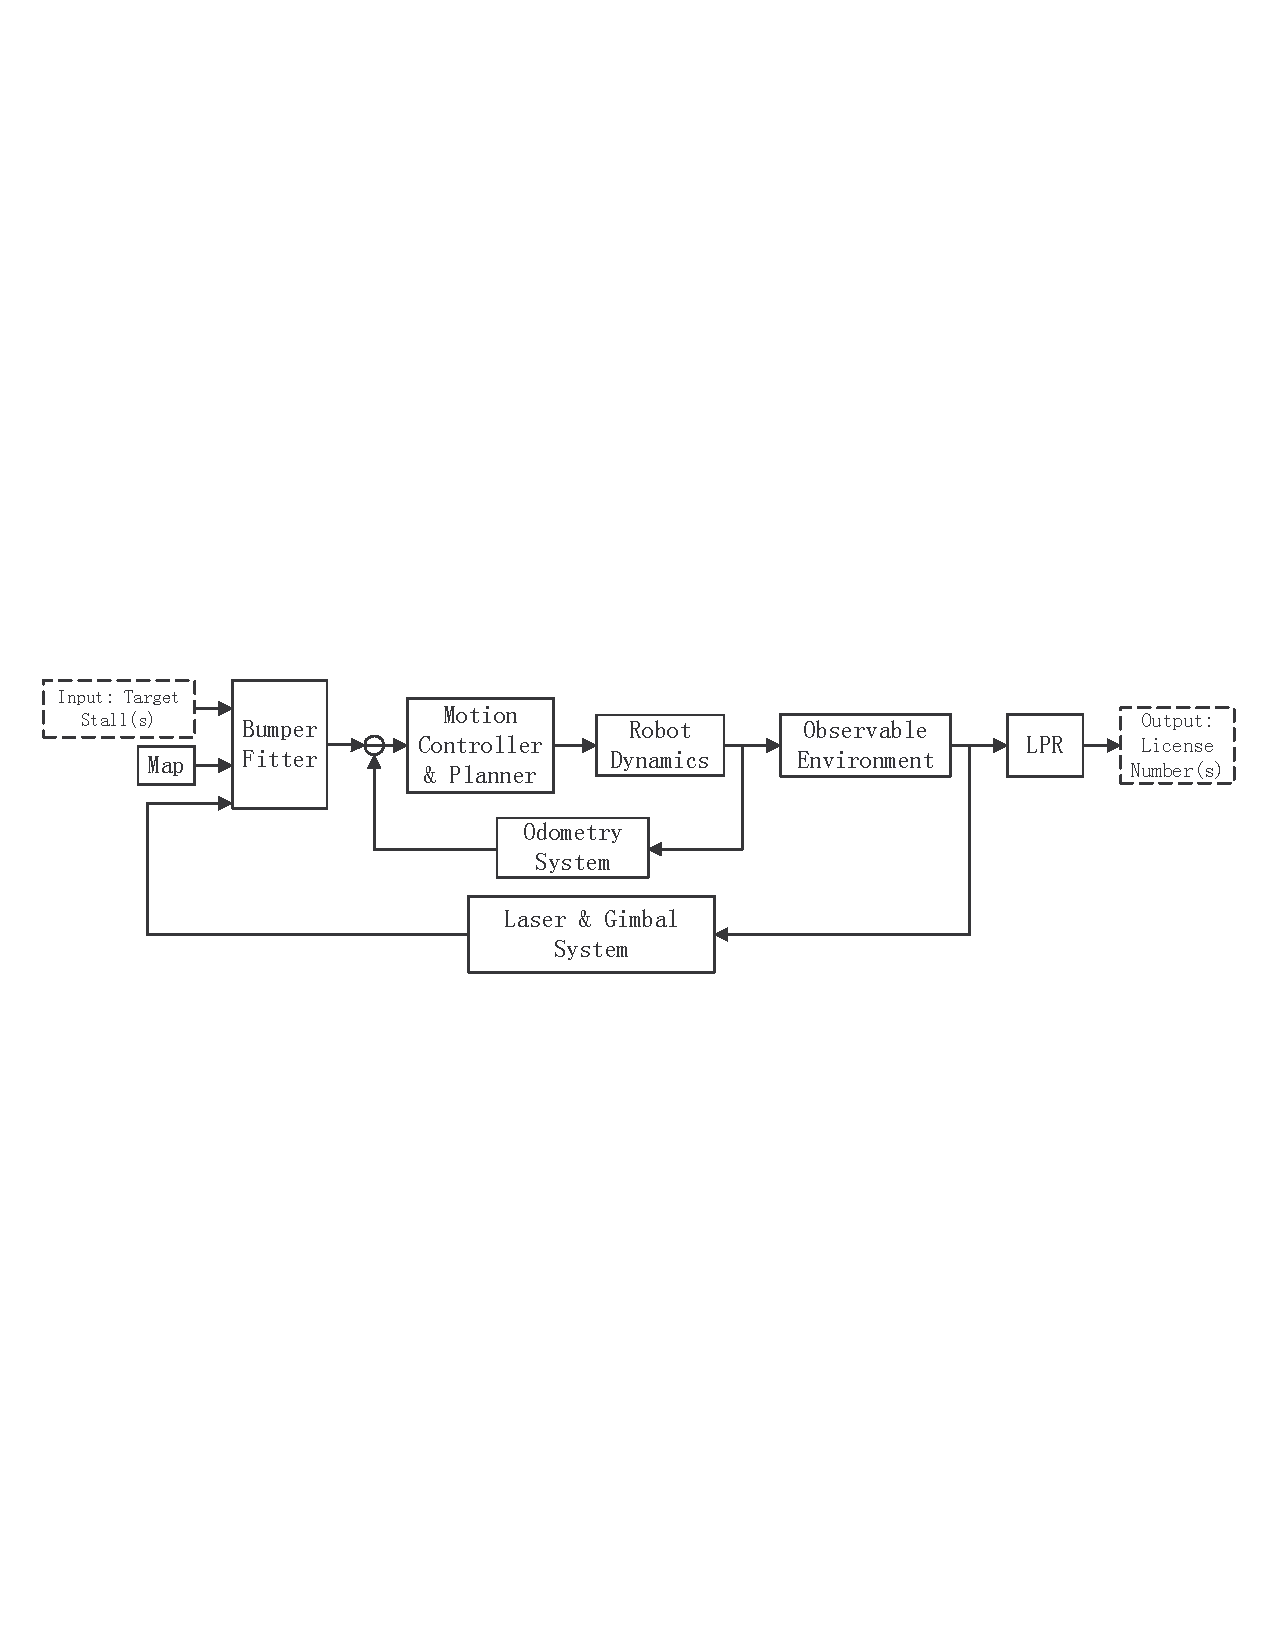
\includegraphics[width=0.9\textwidth]{LaserServoingBlock}
    \caption{Laser servoing system diagram.}\label{fig:sysdiag}
\end{figure}

    Figure~\ref{fig:t4odis} is a picture of T4/ODIS system. T4 is the bigger robot on the left. On the right, ODIS is docking into the elevator of T4. Because T4 is not finished at the time when we wrote this paper, we used T2E robot to simulate T4. Their software architectures are exactly the same, but the hardware are different. For the rest of this paper, we will not distinguish T4 and T2E by default, because the software and sensor system on T2E will be immigrated to T4 without modification. Figure~\ref{fig:t2e} is a picture of T2E. On the left, the 2D laser and gimbal system is mounted in the front of T2E. In middle of the figure, there is a camera header, which contains a infrared (IR) camera, an optical filter, and an illumination system, mounted on the left of T2E. T2E also has many sonar sensors, but we will not discuss them since they are not directly related to the laser servoing task.

\com{Paper structure.}
    Sec.~\ref{sec:plat} will describe the platforms of the laser servoing system: T4/ODIS robot system. The descriptions will cover the following topics: basic configurations of T4, specifications of laser, gimbal, and LPR system, analysis on the height of laser, \t4lpr application, accuracy rate of LPR, and the system architecture. Sec.~\ref{sec:servoing} will focus on the bumper fitting algorithms and its implementations. Based on the analysis on the characteristics of laser data, Hough transform based algorithms, i.e., standard Hough transform (SHT) and sparse Hough transform (SPHT), were implemented on T4. Sec.~\ref{sec:exp} will present the experiment results. Sec.~\ref{sec:con} will conclude the paper.

\begin{figure}[!htb]
    \begin{minipage}{0.45\textwidth}
       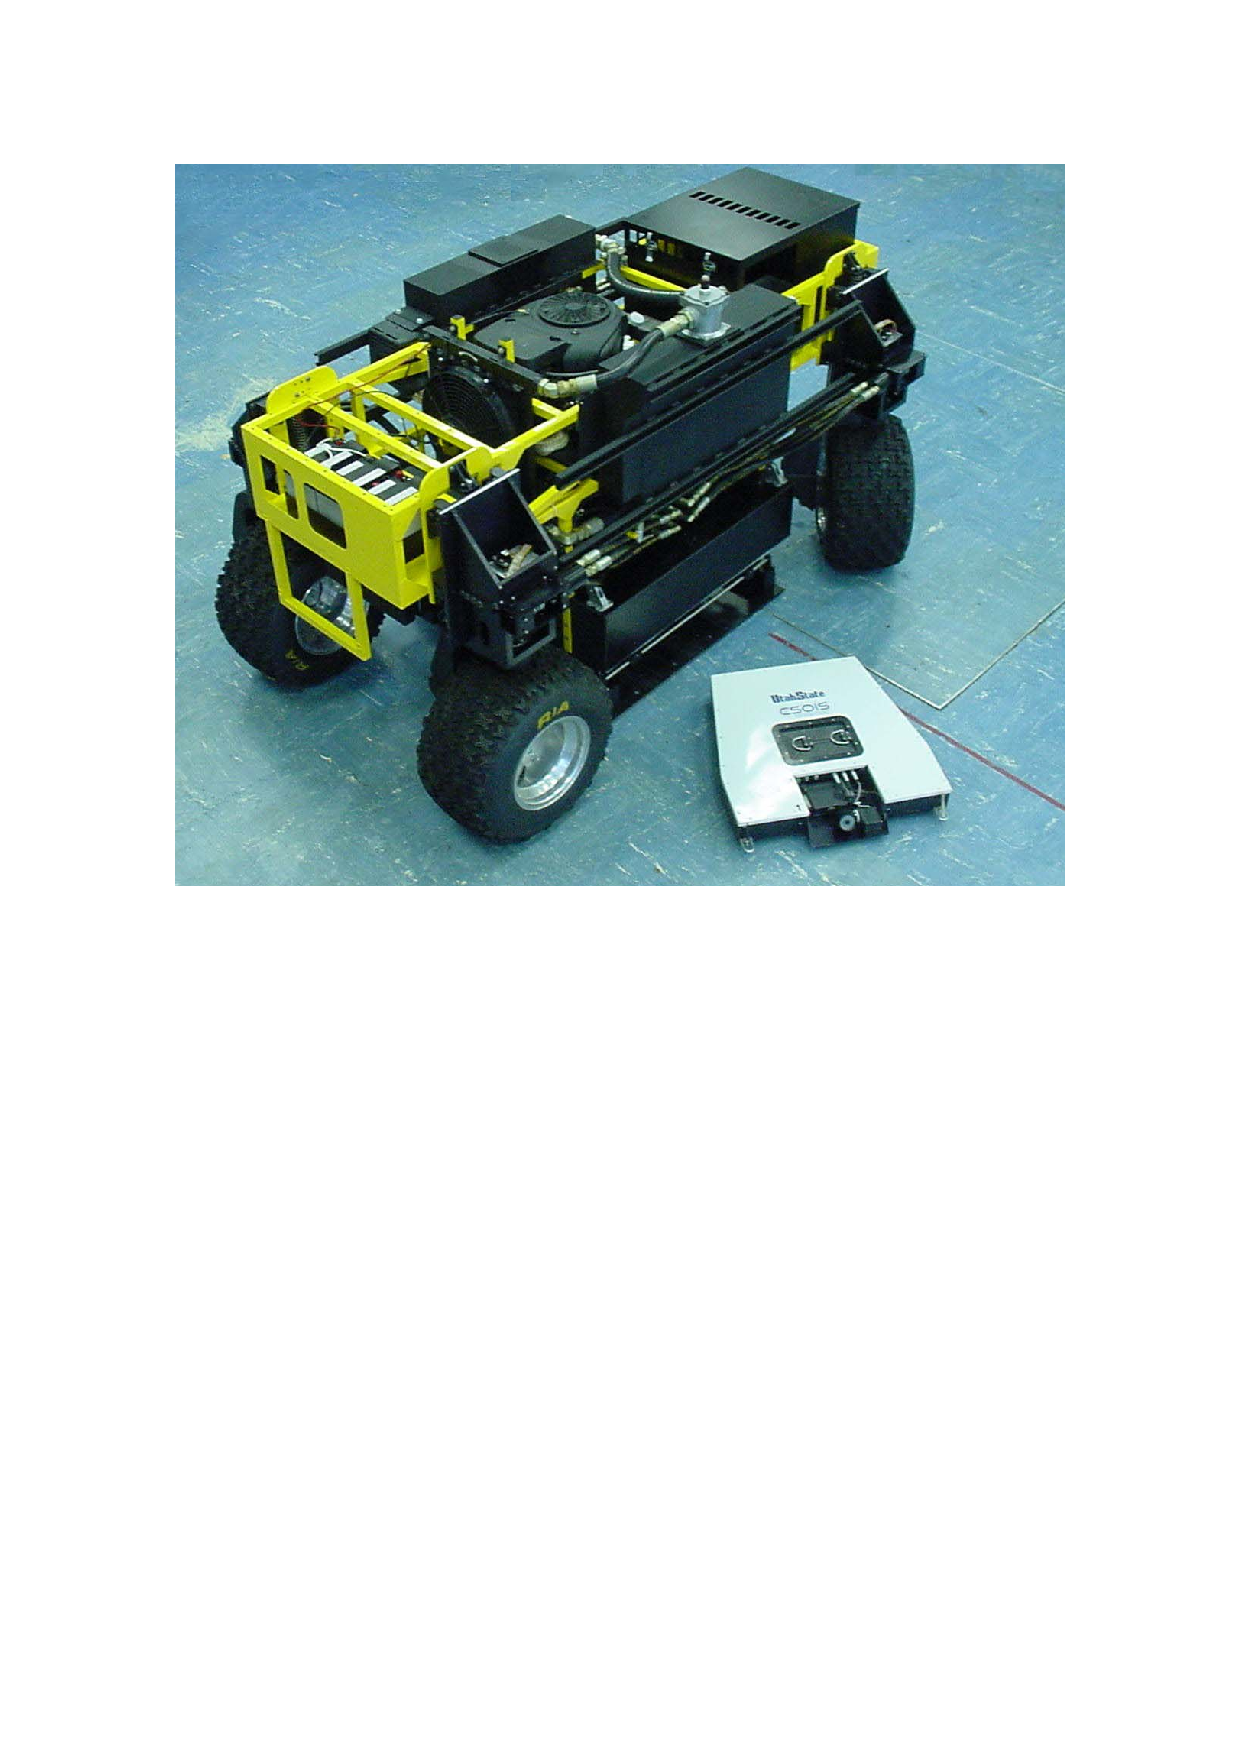
\includegraphics[width=0.6\textwidth]{T4ODIS}
       \caption{ODIS is docking to T4}\label{fig:t4odis}
    \end{minipage}
    \begin{minipage}{0.45\textwidth}
        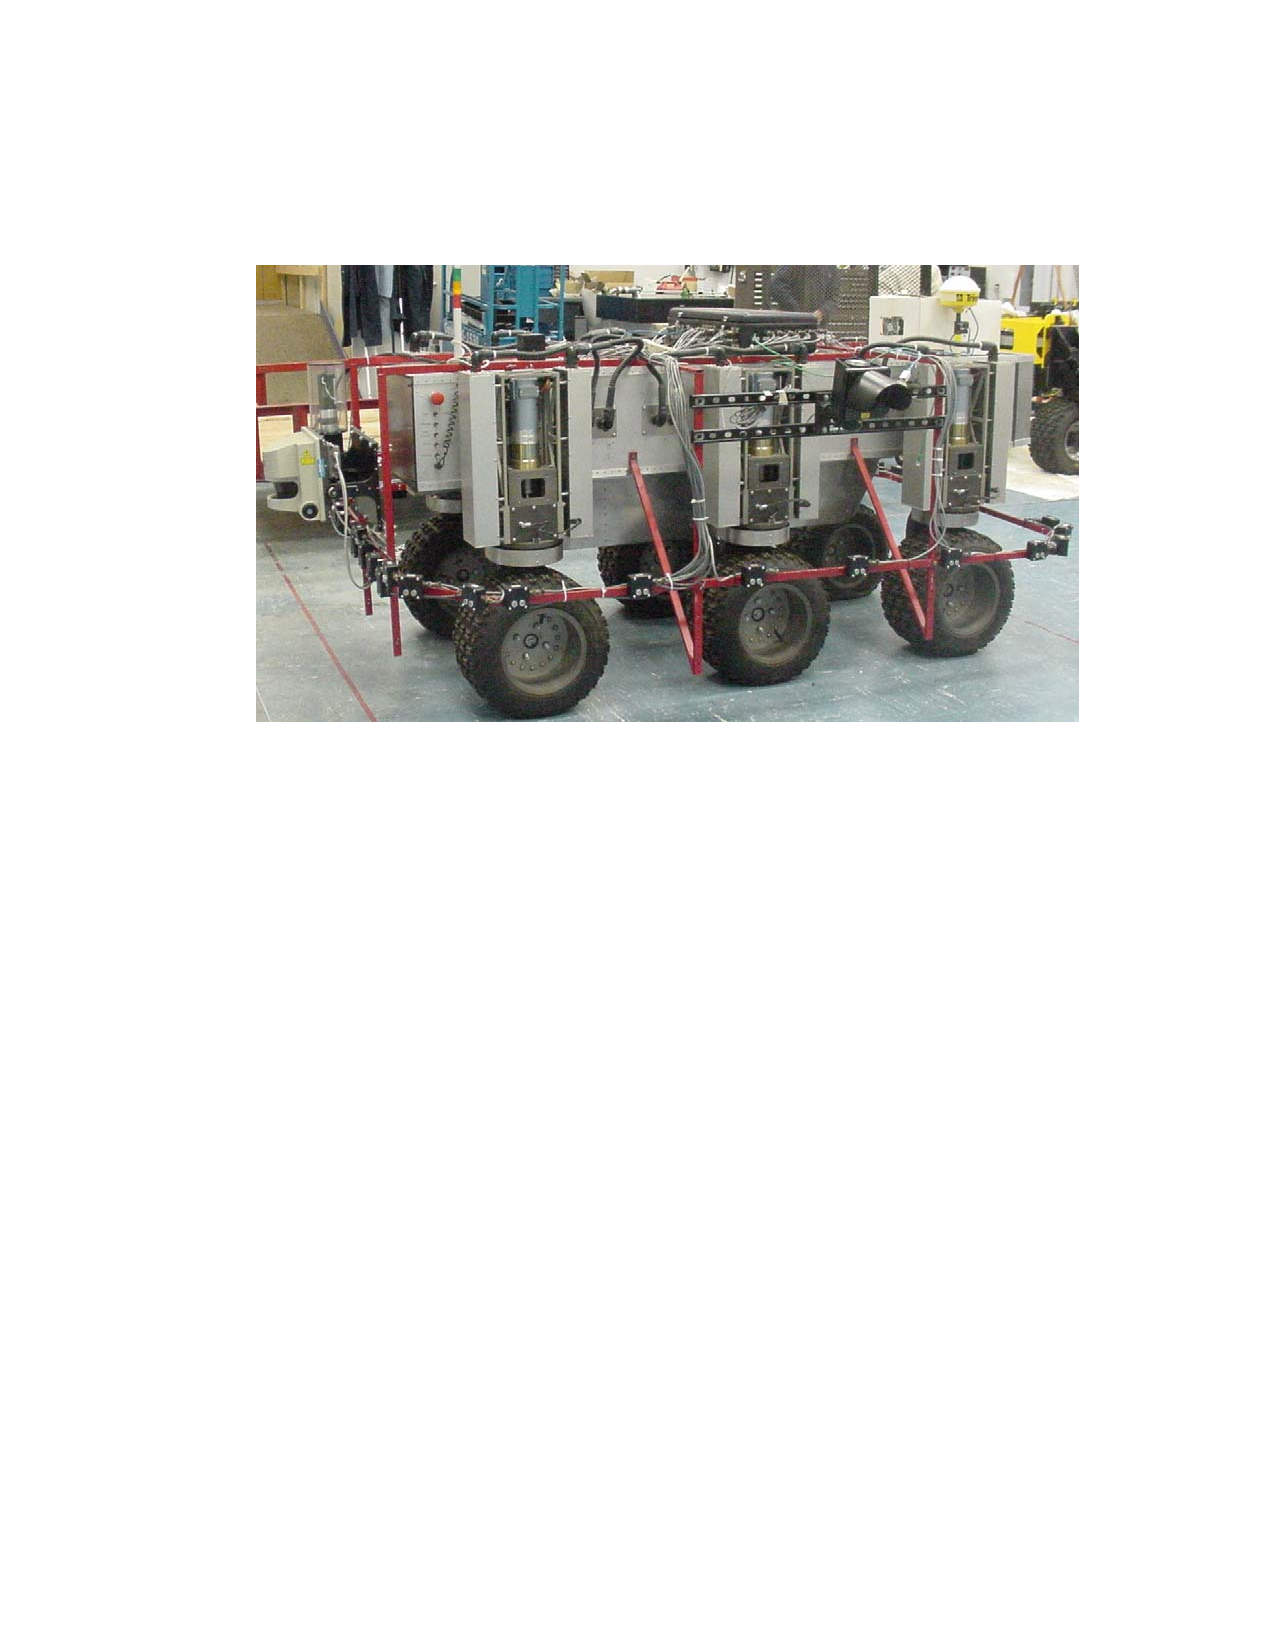
\includegraphics[width=70mm]{T2E}
        \caption{T2E robot, the platform of testing}\label{fig:t2e}
    \end{minipage}
\end{figure}


%If the license of a vehicle is no permitted, T4 will release ODIS from its elevator, and ODIS can go under that vehicle for under chassis inspection. Figure~\ref{fig:t4odis} shows the unfinished T4, which is the larger robot on the left, and ODIS, which is docking to the elevator from the right side. Figure~\ref{fig:t2e} is a picture of T2E. On the left of the picture, a 2D laser and its gimbal system were mounted in front of T2E. In the middle of the Fig.~\ref{fig:t2e}, there is a camera header\com{head?}, which includes a infrared (IR) camera, an optical filter and an illumination system. The LPR used this camera header to take images on license plates for number recognizing.


%    For T4 system, the inspection distance and inspection angle have significant effect on the accuracy rate of the LPR system. In order to enhance the accuracy rate, T4 needs to trigger the LPR system when it is about 3 m to the center of the suspect plate, and perpendicular to it. These requirements have certain redundancy, i.e., the accuracy rate is still acceptable if the inspection distance or orientation are deviated to certain extend. More discussions on the accuracy rate will be presented in Sec.~\ref{sec:LPR}. %Although the accuracy rate under this case is the best, it is too strict for T4. This paper will study on the recognition characteristics of the LPR system, relax the requirements, and still keep the accuracy rate at a reasonable level.
%Because the environment of parking lot is structured dynamic, i.e., the positions of the stalls are known, but the vehicles are dynamic and have unknown position, the parking lot map can not direct T4 to trigger the LPR system at proper distances and orientations.\com{prove?}  Among all the sensors, i.e., 2D laser scanner, sonar, and camera, of T4, the 2D laser scanner is the most suitable sensor for the plate location task. Because, firstly, laser data are range signals that are easy for distance and orientation estimation. These is the fundamental difference between laser and image data. Since the image data are 2D data without distance information, distance and orientation estimation by image is more difficult; secondly, laser is more precise than sonar, and maybe image; thirdly, since the laser scanner sweeps 180$^\circ$ every 100 ms, it is fast enough for this real-time application. So, we uses 2D laser data to estimate the positions of license plates to guarantee the LPR accuracy rate. In practice, since the licence plates are too flat that it is difficult to identify it by the laser ranger data, we developed an algorithm to fit bumpers and use their distances and orientations as the reference signals for the motion control of T4. As we described above, since the LPR system has redundances on both of the inspection direction and orientation domains, we took the distances and orientations of bumpers as approximations to that of the license plates. This approach was proved reliable in practice.

\section{Testing Platform}\label{sec:plat}

\subsection{T4 System Overview}
\com{system architecture}
    The modules of T4 and the workstation that related to the laser servoing task were plotted in Fig.~\ref{fig:bfitarch}. On this figure, those blocks with shadows are the concepts in the software domain, and those without shadows are physically existing hardware. All the blocks in the left dash line box are installed on T4, and those on right are on the workstation side. This figure does not distinguish between hardware connection and software coupling. Any line in the figure that has a hardware block on one of its two sides is a physical wire, and the line connects two software blocks is a software coupling. A software coupling might be a ``calling'' between functions, or a communication channel among different threads.

    T4 has three embedded computer systems called ``master node,'' ``sensor node,'' and ``LPR node'', respectively. Most of the functions were implemented on the ``master node,'' including the supervisory task controller (STC)~\cite{Shah02}, a map database, and different threads that dedicated to individual tasks. ``sensor node'' mainly pre-process the raw sensor data in real-time, then send the result to the workstation via the master node. Without the pre-processing, the master node might not have enough computation power to process in real-time. ``LPR node'' is dedicate to the \t4lpr application, which can grab images from the LPR header, identify license numbers, and send results to the workstation via master node. These three nodes are connected by TCP/IP ethernet connections via a hub, which is also connect with a wireless TCP/IP node that communicates with the other node on the workstation side. The odometry system that connected to the sensor node can estimate the robot's position and orientation in real-time. As shown in Fig.~\ref{fig:sysdiag}, odometry information performances as a feedback of the inner loop in the system.

    In the master node, STC is linked with a dashed line block that contains ``bumper fitting thread,'' ``awareness thread,'' and other threads, which means the STC can communicate with each of these threads individually. The bumper fitting thread, together with the ``LaserComm'' thread and the pre-process module on the sensor node, are the ``bumper fitter'' in Fig.~\ref{fig:sysdiag}. Although the bumper fitter is not physically connected to the GUI, which is the reference input or map, they are connected in logic, because many other modules, such as hubs, perform as relays of the communication flow.

    The awareness thread is that danger avoidance thread that can use laser and sonar data\footnote{The communication channel between the awareness thread and sonars is not shown in Fig.~\ref{fig:bfitarch}, because it is not directly related to the laser servoing system.} to build map of surrounding environment in real-time and halt the vehicle in emergence~\cite{MaHIMM}. Because the danger avoidance has higher priority than the laser servoing, we must consider the requirements together in order to reduce the chance of conflictions when the awareness thread has to preempt the bumper fitting thread and halt the laser servoing procedure. The result of this consideration is that the 2D laser must scan horizontally at a proper height. The details will be presented in Sec.~\ref{sec:LaserH}.

    The ``xxxComm'' blocks are functions of the communication thread. They share the same IP address, but have different TCP sockets. The reason for separating them from task threads, such as the bumper thread, is that the operating systems (Linux and Windows 2000) of these three nodes are not real-time operating systems, but the application requires real-time capability, i.e., each node has to process received data packets in time, otherwise the robot might be in danger. In the system, light duty communication thread is dedicated for packet buffering, so that the packet losing is prevented as much as possible.

    The \t4lpr application executing on the LPR node is based on the \seecar DLL\footnote{``DLL'' stands for the dynamic link library on Microsoft Windows. \seecar DLL is a module of the \seelane system.}, which returns a license number after received a image of a license plate. On the LPR node, there is a frame grab card that can record signal from the LPR header into bitmap format. The \t4lpr application transfers these images to the \seecar DLL for identification, and send the result to the ``LPRComm'' thread with a TCP/IP connection. In order to enhance the accuracy rate, \t4lpr can take up to 10 images of one license and consider the results comprehensively to get the best fit license number. In the testing of this paper, \t4lpr took 5 images for each license.

    On the workstation side, the system is simplified as GUI and CSI. The GUI is an integrate information environment that can display the information, such as position and latest found license number, of T4 and ODIS on the screen. At the same time, it can also receive operations from the keyboard and the mouse, and transfer them to the CSI. The CSI can compile these operations into STC compatible ``command units'' and send them to T4 and ODIS via the wireless connection. The details are out of the range of this paper.

\begin{figure}[!htb]
\centering
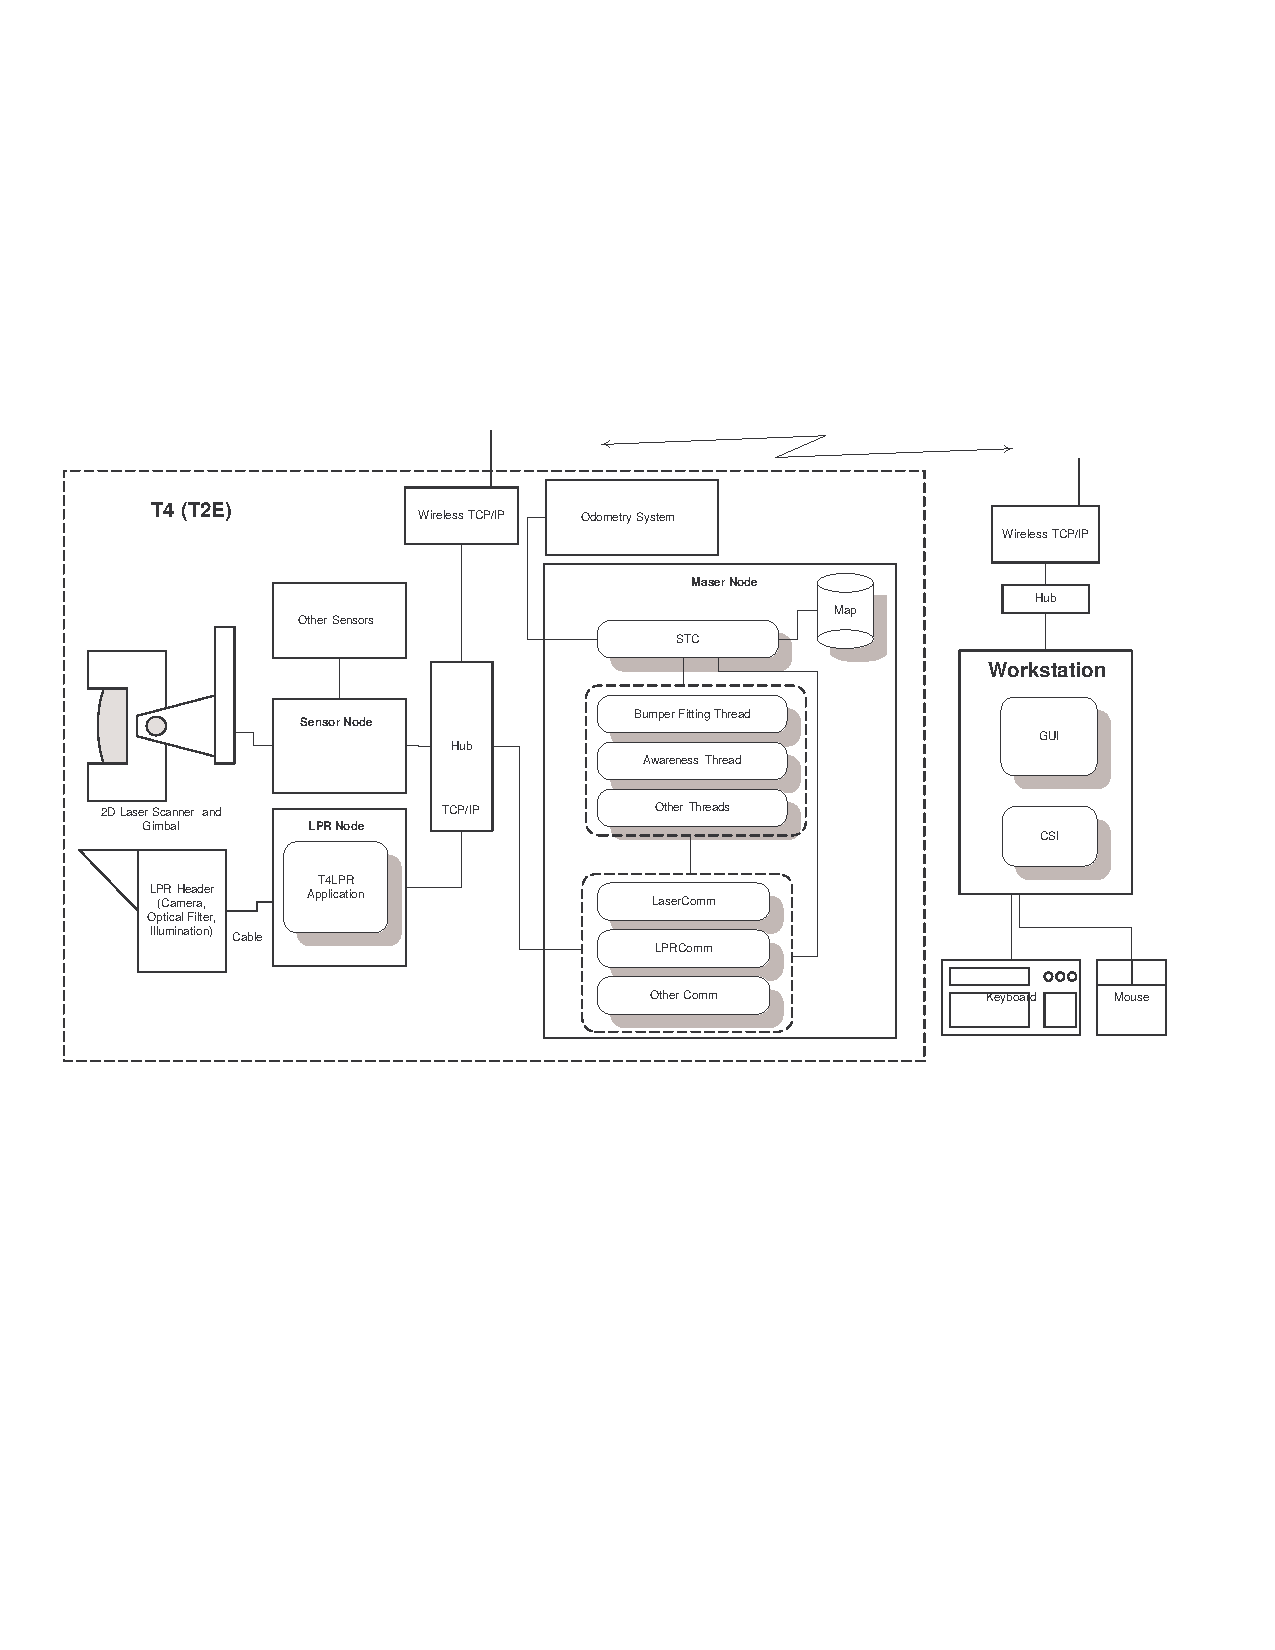
\includegraphics[width=0.9\textwidth]{BumperFitArch}
\caption{System architecture of bumper fitting}\label{fig:bfitarch}
\end{figure}

\subsection{LPR Checking Mission}
\com{T4 and T2E tasks: how to check LPR}
    The executing procedures of a typical license plate checking mission are illustrated in Fig.~\ref{fig:track}. On the left, there are stalls and several cars in them. T4 started from the lower right position, and moved upward follow the dash arrow. The semicircle in front of T4 represents the 2D laser and gimbal system. The arrow on the left of T4 is the camera header. The ``bumper box'' is drawn in dashed line on Fig.~\ref{fig:track}.  Each ``bumper box'' is a rectangular region of 1/4 of the length of a stall, and with the same width of the stall. Since the stalls are static, these bumper boxes are also static, i.e., they are well known before the mission starts. Cars are illustrated by white boxes with dark edges, which represent the bumper. Cars are dynamic objects in the sense that their positions are not known before the mission, but this does not imply they are moving during the checking license mission. Instead, we assume they will not move once T4 started its mission. The numbers in the figure represent the different position on the tracks of T4. The comments for each position are the followings:
    \begin{enumerate}
    \item After T4 just finished the one license checking task for the car in \stall{1}, new commands came from the workstation side. The planer of T4 checked map and the current position measured by the odometry system, then decided to go straight forward. Because the LPR system is not sensitive to the inspection distance, which will be explained in Sec.~\ref{sec:LPR}, T4 just went straight in order to simplify the system. T4 queried the map and get the positions the associated bumper boxes of the next three stalls, i.e., \stall{2} to \stall{4}, on its left. Every 100 ms, when a new set of 2D laser data arrived, T4 fitted the bumpers by the data points that fell into these bumper boxes.
    \item With more and more laser data came in, the fitted bumper changed and was closer to the real bumper. When T4 moved from the position ``1'' to the position ``2,'' the fitted bumper changed from \texttt{B1} to \texttt{B2}. The position 2 is defined as the intersection on the extension of the common edge of \stall{1} and \stall{2} and the robot's track. At the position ``2,'' T4 inquired the best fitted bumper line from the bumper fitting thread, and the position ``3'' is the best inspection position according to the fitted bumper.
    \item At position ``3,'' T4 triggered the LPR system, wait for 5 sec., report the result to the workstation, and delete the information of the bumper box in \stall{2}. Then, T4 started to track the stall above \stall{4}, and move toward position ``4.''
    \item At position ``4,'' T4 checked the fitted bumper line and set the target position as ``5.''
    \item At position ``5,'' T4 did the same job as it did at ``3.'' Follow these procedures, T4 moved on until it finished all the stalls.
    \end{enumerate}



\begin{figure}[!htb]
    \centering
    \begin{minipage}{0.7\textwidth}
        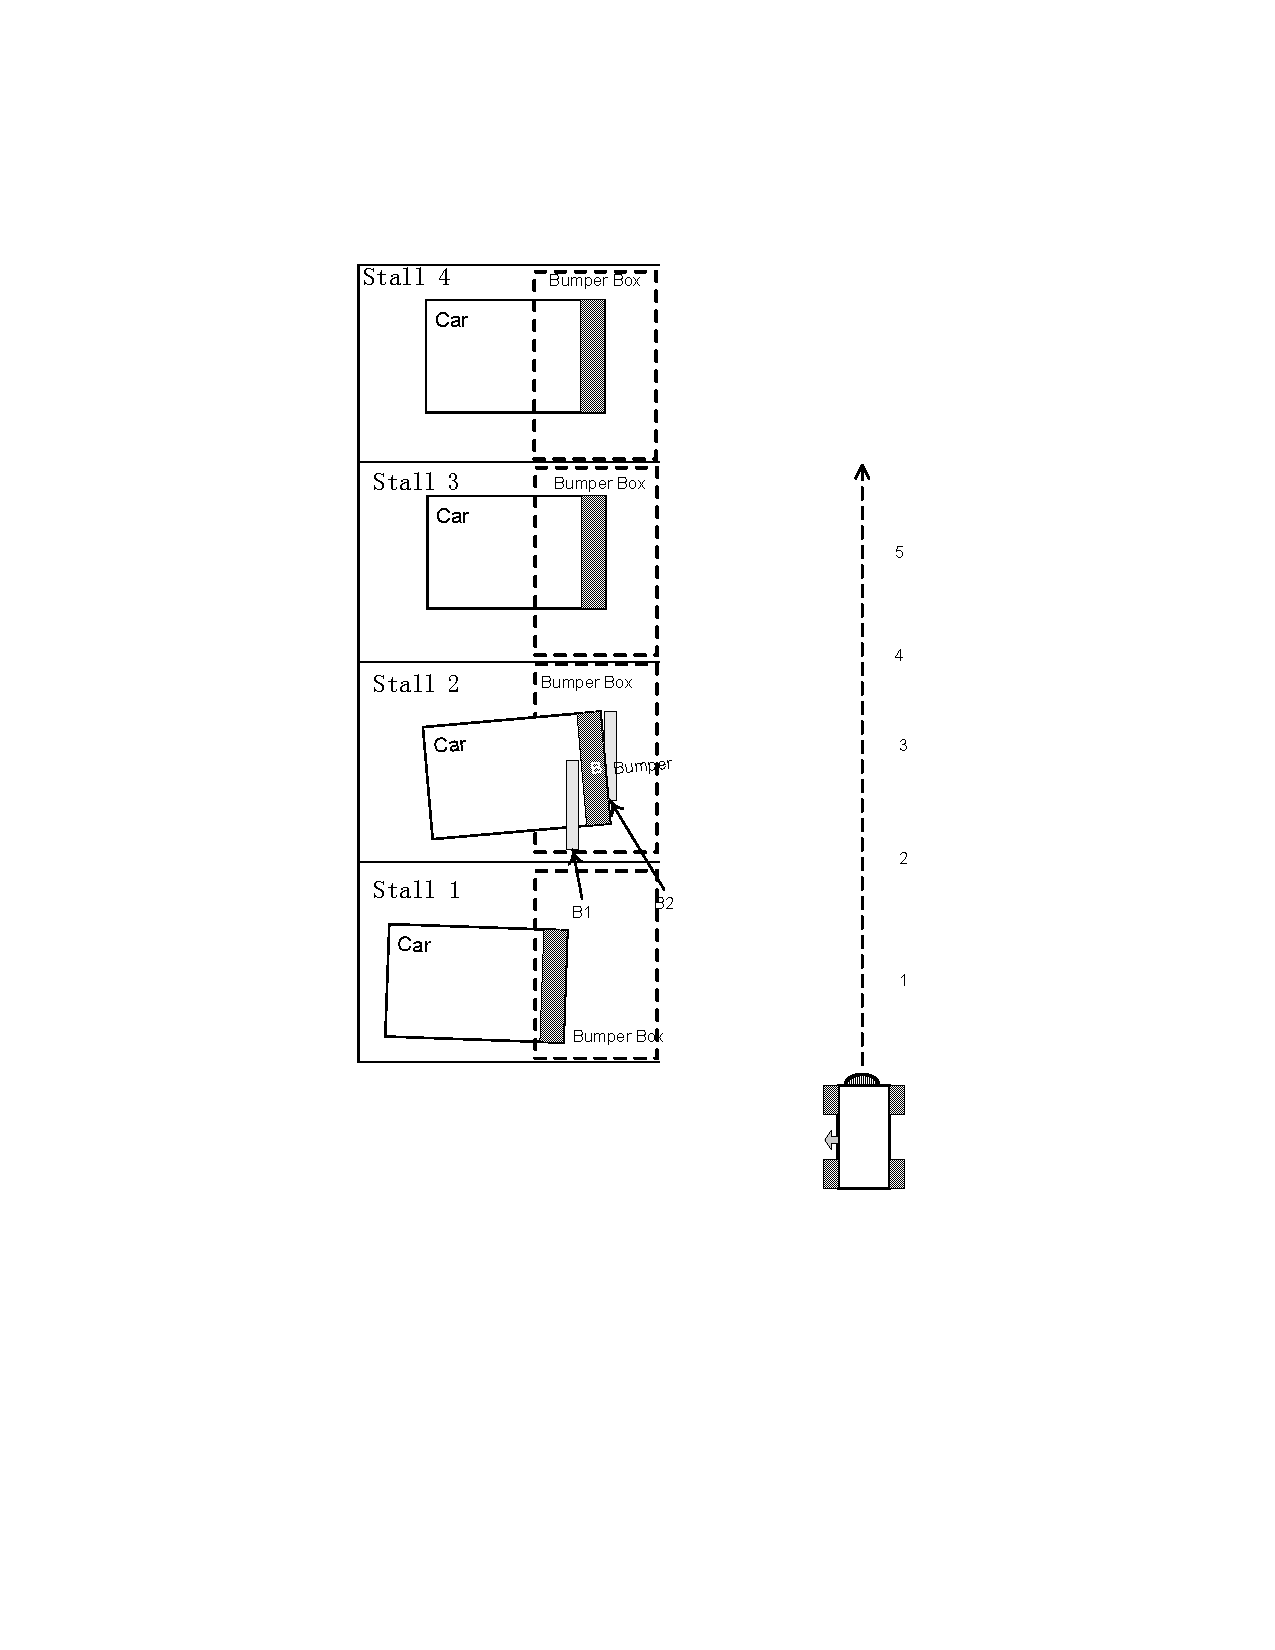
\includegraphics{Track}
        \caption{LPR checking when moving straight.}\label{fig:track}
    \end{minipage}
%    \begin{minipage}{0.45\textwidth}
%        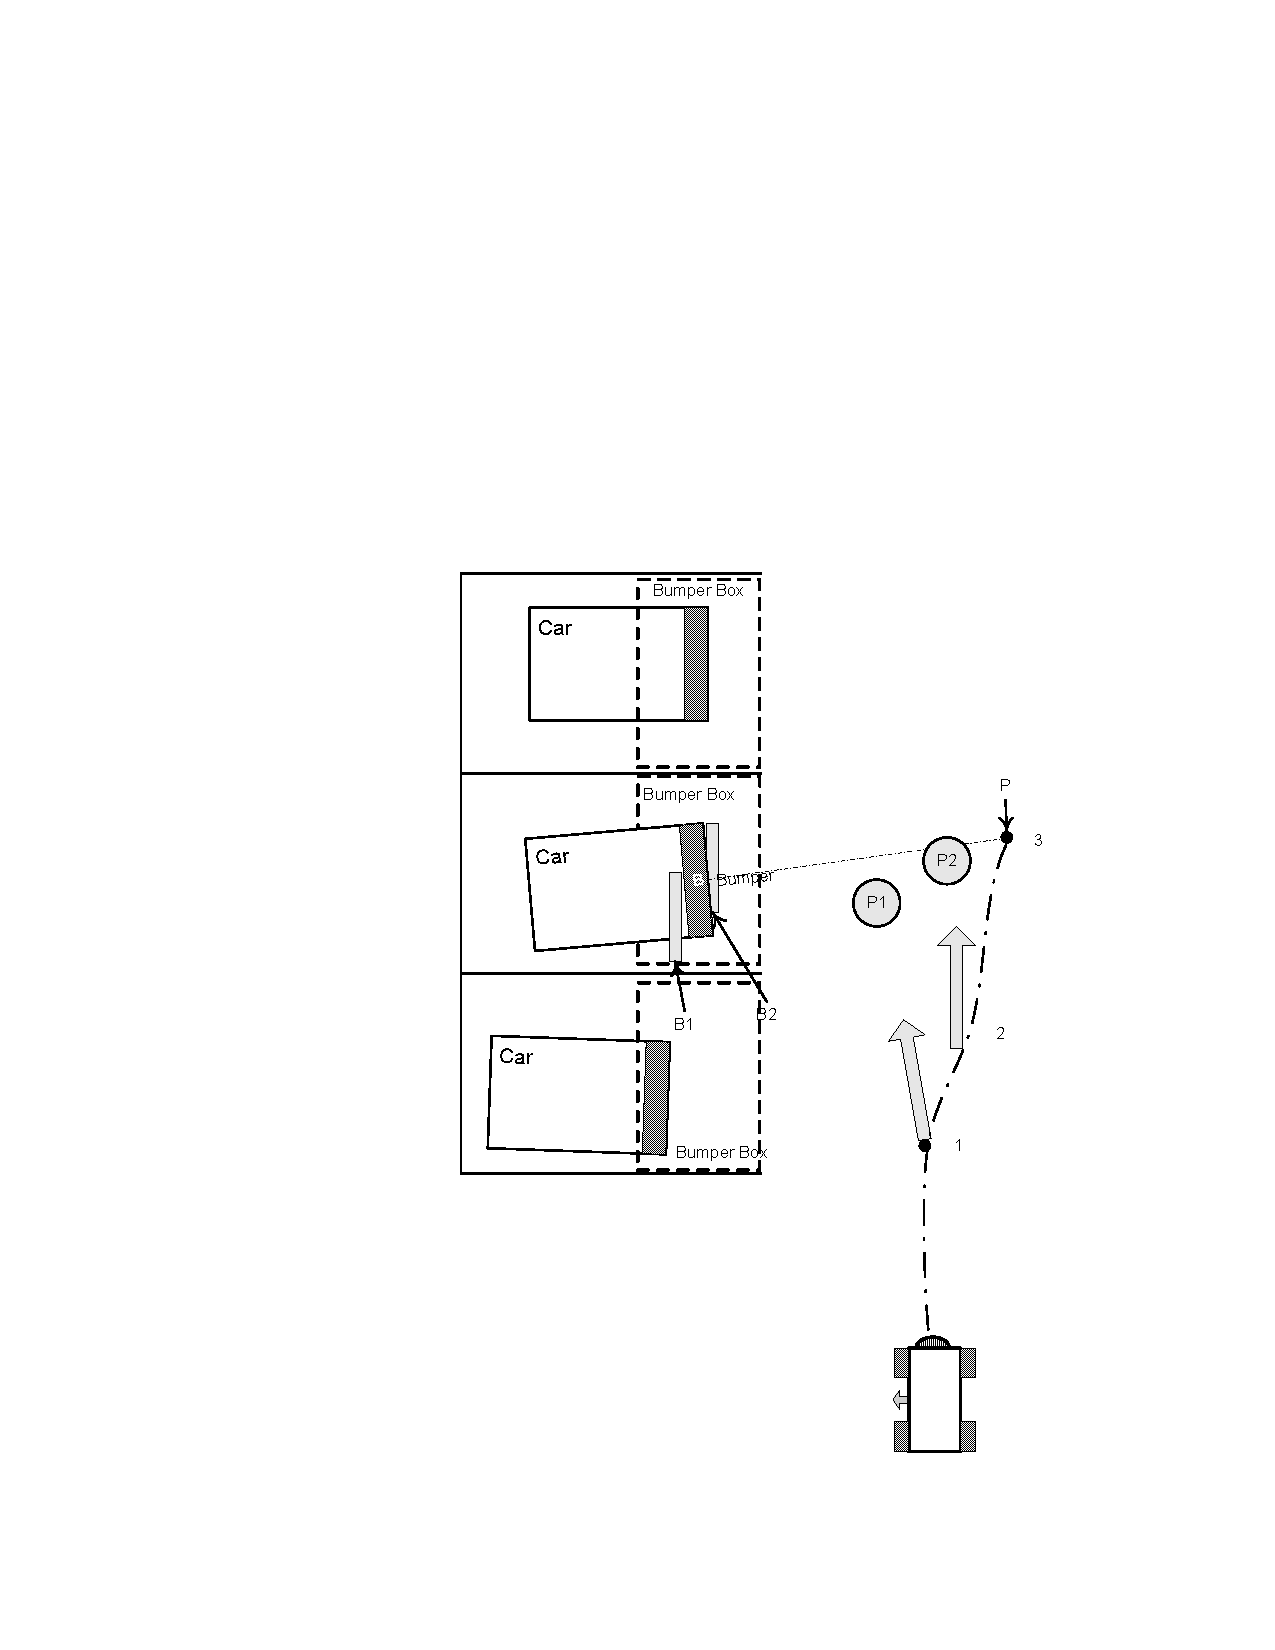
\includegraphics{Tracking}
%        \caption{LPR checking when moving through curve}\label{fig:Strack}
%    \end{minipage}
\end{figure}

\subsection{2D Laser Scanner and Gimbal System}
\subsubsection*{Specifications}\label{sec:spec}
\com{2D Laser: type, resolution, detection distance}
    The specifications of the 2D laser scanner is listed in Table~\ref{tab:2D}, and Table~\ref{tab:gimbal} is the specifications for the gimbal system.
\begin{table}[!htb]
    \begin{minipage}[t]{100mm}
    \caption{Specifications of SICK 2D laser scanner.}\label{tab:2D}
    \begin{tabular}{|p{30mm}|p{60mm}|}%0.7\textwidth}|}
        \hline\hline
        % after \\: \hline or \cline{col1-col2} \cline{col3-col4} ...
            Type & Sick LMS 220 \\ \hline
            Dimensions & (352 $\times$ 228.5 $\times$ 266mm), 9kg \\ \hline
            Distance Error & $<$ 1cm \\ \hline
            Angular Resolution & 0.25$^\circ$ / 0.5$^\circ$ / 1$^\circ$ (selectable) \\ \hline
            Scanning Angle & 180$^\circ$ \\ \hline
            Detection Range & Maximum 80m, and 10m for 10\% reflectivity objects \\ \hline
            Response Time & 53ms/ 26ms / 13ms (resolution dependent) \\ \hline\hline
    \end{tabular}
    \end{minipage}
    \begin{minipage}[t]{0.45\textwidth}
        \com{Gimbal: speed, angle range, coordination system}
%        \begin{table}
        \caption{Specifications of gimbal system.}\label{tab:gimbal}
        \begin{tabular}{|p{20mm}|p{40mm}|}\hline\hline
        Type & Self made \\ \hline
        Tilt Angle & -90$^\circ$ to 45$^\circ$ (upward is positive)\\ \hline
        Resolution & 1$^\circ$ \\ \hline
        Speed      & 45$^\circ$/sec. \com{check!} \\ \hline\hline
        \end{tabular}
%        \end{table}
    \end{minipage}
\end{table}



\subsubsection*{2D Laser Height}\label{sec:LaserH}
\com{Vehicle bumper height}

    Figure~\ref{fig:vH} plots heights of some vehicles. Each vertical line in this figure represents one vehicle. The short bars of top of these lines is the bottom of the window. Since the laser beam can go through the glasses of the windows, and ``see'' inside of the vehicles, the data points higher than this line can not indicate the position of the license plate of a vehicle. Between the first bars and the second bars, which represent top of bumpers, are the engine covers. Although the laser data points fall in these regions will be further than the position of the bumpers, the error will be less than those points above the first bar, since the length of the engine covers are limited. From the second bars to the third bars are the bumpers. Data points in this region can indicate the exact distances and orientations of bumpers.

    For the bumper fitting algorithm, the desired height of the 2D laser scanner is between the second bar and the third bar, and the desired tile angle is 0. This configuration can greatly simply the bumper fitting algorithm and the easily guarantee the real-time property.

    Consider the case when the laser scanner is mounted higher than the bottoms of windows. Then the title angle has to be adjusted according to the distance between T4 robot and the target vehicle in order to shine the laser beam roughly to the bumper and measure the orientation. One disadvantage of this configuration is the limited speed. As shown in Tables~\ref{tab:2D} and \ref{tab:gimbal}, the 2D laser scanner is very fast compared with the gimbal system. So it is better to continuously scan the laser beam than adjust the title angle. Another disadvantage of the configuration is the complexity. For this approach, the laser will ``see'' the ground, bumpers, engine covers, windows, and might ``see'' some thing inside the windows, etc. Then the bumper fitting algorithm has to segment data points, and fit the bumper only. On the other hand, if the title angle is 0, the data points are actually in 2 dimensions, since the differences between their heights are neglectable.

    For the case when the 2D laser is mounted lower than the bottom of bumpers, the 2D laser and gimbal system might be damaged by stones on road. Still, since the tilt angle is positive, and the measured data are in 3 dimensions, the complexity due to segmentation is still not avoidable.

    So, for the requirements of the bumper fitting algorithm, the desired height of the 2D laser is about 28in. But before we chose this height, we need to consider constrains from the awareness thread~\cite{MaHIMM,BahlMultiRobot} and localization thread~\cite{Song02,BahlMultiRobot}, since these two threads also need laser data.

\begin{figure}[!htb]
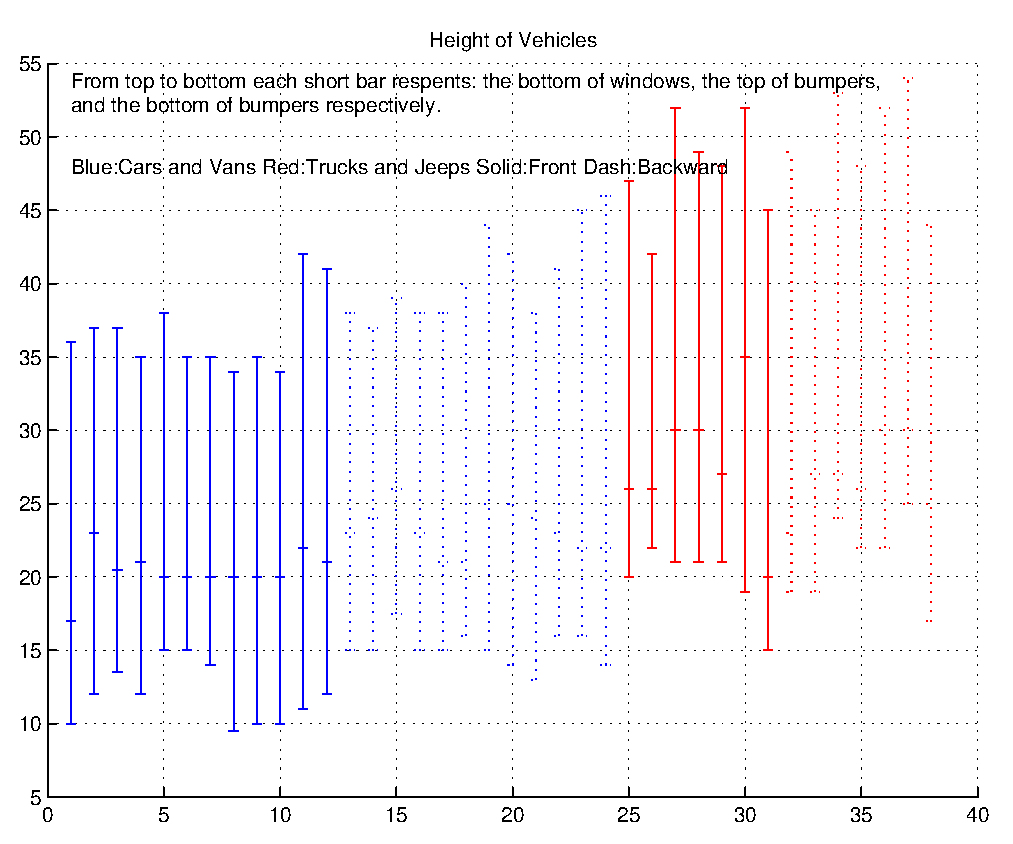
\includegraphics{VehicleHeight}
\caption{Vehicle heights in a parking lot.}\label{fig:vH}
\end{figure}

\com{Constrains: localization and awareness thread}
    The awareness thread can process laser and sonar data in real-time, build a HIMM map, estimate positions of potential dangerous objects, and halt T4 robot if necessary. In order to detect objects as far as possible, the best laser tilt angle for the awareness thread 0, which means the laser should scan horizontal. Since security is more important than any mission, the awareness thread has the highest priority which enable it to preempt laser/sonar data and the gimbal control. If 2D laser is mounted on a certain height such that horizontal scanning can support both awareness thread and the bumper fitting, then resource confection is reduced, and system security is improved. The localization thread can locate T4 and calibrate its odometry system. There are two kinds of landmarks in the parking lot: curbs and lampposts, and two types of localization strategies: real-time localization, i.e., locate while moving, and static localization, i.e., stop and locate. For the static localization, the landmark can be a curb, thus the tilt angle of the gimbal system will change inside a range and get a 3D point cloud for the localization procedure~\cite{Song02}. It has no confliction with the bumper fitter, since the bumper fitting algorithm does not need to work when T4 stops. For the real-time localization, it is still on development. We propose to keep the title angle as 0 in order to  accommodate the laser servoing system.

\com{Final results}
    According to the above considerations, the 2D laser is mounted at 28 in with default tilt angle as 0.

%\subsubsection*{Laser Communication}

\subsection{LPR System}\label{sec:LPR}

\subsubsection*{LPR System Specifications}
\com{Type, hardware, software list. Claimed specifications}
    The LPR system including software and hardware, on T4 is based on the \seelane system of Hi-Tech Solutions Inc.. On the software part, the \seelane system includes a license identification DLL called ``\seecar DLL,'' and an GUI application call ``\seelane application,'' which is not installed on T4 because it can not communicate with ``LPRComm'' on the master node. Instead, we programmed an application called \t4lpr that calls \seecar DLL and communicates with the ``LPRComm.'' The hardware of the \seelane system includes a camera header, which integrated an IR camera, an optical filter, and an illumination system, a frame grab card, cables, a license plug\footnote{The license plug is a plug on the parallel port that enables the \seecar DLL.}, and a PCI I/O cards that controls the level of illumination. The illumination system has three levels of brightness, and the \seecar DLL prefers to get images of different levels, thus the identification result is more reliable. Because the embedded computer on T4 has no PCI slot, the testing of this paper is based on constant illumination level. 
%\com{Installation on T2E}
%\subsubsection*{\t4lpr Application}
%\com{Runs on master node as a TCP/IP server for the ``master''}
%\com{Multi mode and single mode.   How does the first one improve the accuracy rate}

\subsubsection*{The Accuracy Rate of LPR}
\com{Factors that effect the accuracy rate: sunshine, mode, distance, angle. }
    There are several factors that effect the accuracy rate of the LPR system: sunlight, distance, angle, and identification mode. 

    If there is no protection against the sunshine, the accuracy rate of the LPR system can be virtual zero. To reject the disturbance of the sunshine, we chose 940 nm narrow band IR optical filter, and the illumination system with the same wave length. Although the sunshine has much more energy than the illumination system for all the spectrum, the bandwidth of the illumination is very narrow, thus in this specific bandwidth the illumination is much stronger than the sunshine. Then, the disturbance of the sunshine is not significant. Because most of the US licenses are reflective to IR, while the paint of the vehicles and backgrounds, etc., are non-reflective, so the license plates are very bright compared with the dark backgrounds in the IR images. In Fig.~\ref{fig:LPRimg}, the image on top was taken with an optical IR filter, while the lower one was taken without the filter. The accuracy rates on the images with IR filter are much higher, since here is not many objects in this type of image to disturb the license identification procedure. 

\begin{figure}[!htb]
    \includegraphics{IRImg}
    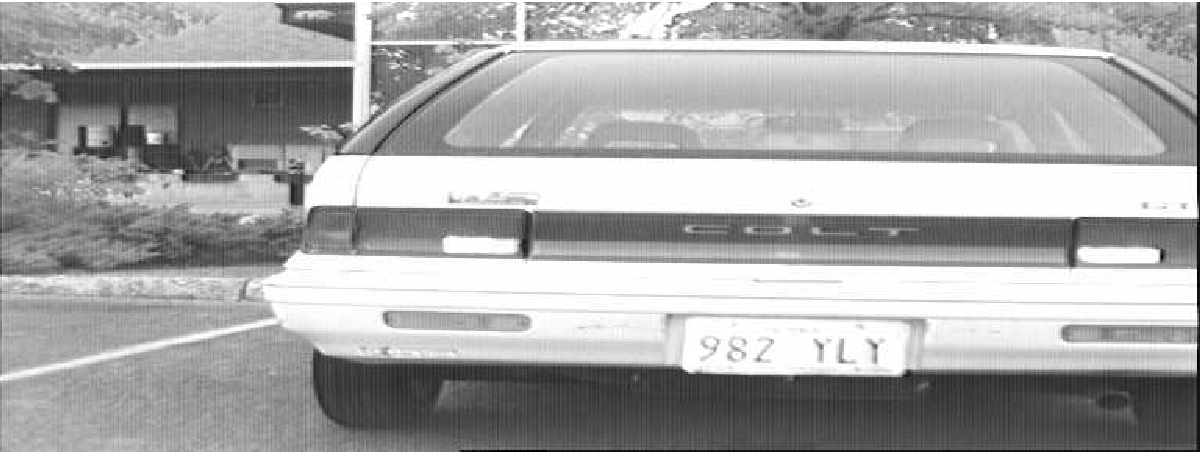
\includegraphics{NoIRImg}
    \caption{Images with and without IR optical filter}\label{fig:LPRimg}
\end{figure}
    
    The LPR system has ``single mode'' and ``multiple mode.'' The former one implies the \t4lpr application returns one license number per image. In the latter mode, the \t4lpr may take up to 10 images, consider the identification result of each one, and return one best fit number in the end. After field testing, we chose the multiple mode with 5 images per identification. 
    
    See Fig.~\ref{fig:LPRang}. D is the center of a bumper, where normally is also the center of the license plate. The segment CD is perpendicular to the bumper. Then, CD is the inspection distance and $\angle$CDA is the inspection angle. While the distance CA is increasing, the accuracy rate of the LPR system firstly dropped, then became zero, because part of the license was invisible. Figure~\ref{fig:LPRacc} has two plots: the upper one is the accuracy rate vs. inspection angle $\angle$CDA, the lower one is the accuracy rate vs. inspection distance CD.\com{demo plots now!} According to these testing results, the positioning angular resolution for LPR should be $\pm$9$^\circ$, and the positioning distance resolution be less than $\pm$50cm. 
    
    The inspection distance and angle are important to the mobile applications, such as robots. By default, \seelane system used a 16mm focus lens whose suggested inspection distance is 8m. However, due to the limitation of the lane width of the parking lot, the common inspection distance of T4 is about 3m. So we replaced with a 9mm lens instead. Easy to see, the license images of \t4lpr system is larger than the suggestion. It is observed in the field testing that the accuracy rate is not very sensitive to the inspection distance compared with the inspection angle. 
    
\section{Laser Servoing Techniques}\label{sec:servoing}

\subsection{Mission Requirements Analysis}
\com{List the requirements from LPR}
    The basic requirements on the bumper fitting algorithm are: fast, progressive, and robust. The algorithm must be able to fit bumper in real-time on an embedded computer, whose computation capability is limited. Progressive is actually derived from the requirement of ``fast.'' Because each 100ms the 2D laser scanner can sweep once and get new data, it is inefficient if the algorithm has to fit again from beginning every time new data come. So the feature of progressive is important. Robust in also an important issue. If the fitting result is wrong, the planner might try to direct the robot to ``run over'' other vehicles. Although there is an awareness thread that supposed to prevent collisions, a ``misleading'' bumper fitter still might lead the robot system to unpredictable dangerous states. Before we chose the fitting algorithm, we use the laser scanner collect 3D data with the tilt angle swept between $\pm$30$^\circ$. After cropped data points farther then 9m, the result of them were plotted in Fig.~\ref{fig:nearpts2}. This figure demonstrated that the laser beam might go through the windows and ``see'' inside a vehicle. (look at the van on right.) Though the height of the 2D laser scanner was carefully chosen such that the possibility of ``see'' though windows is very small, it is still a consider in the algorithm selection due to its high demand on the safety. Another kind of disturbance that did not shown in this plot is pedestrians. They might walk in the bumper boxes and greatly interference the bumper fitter. 

\begin{figure}[!htb]
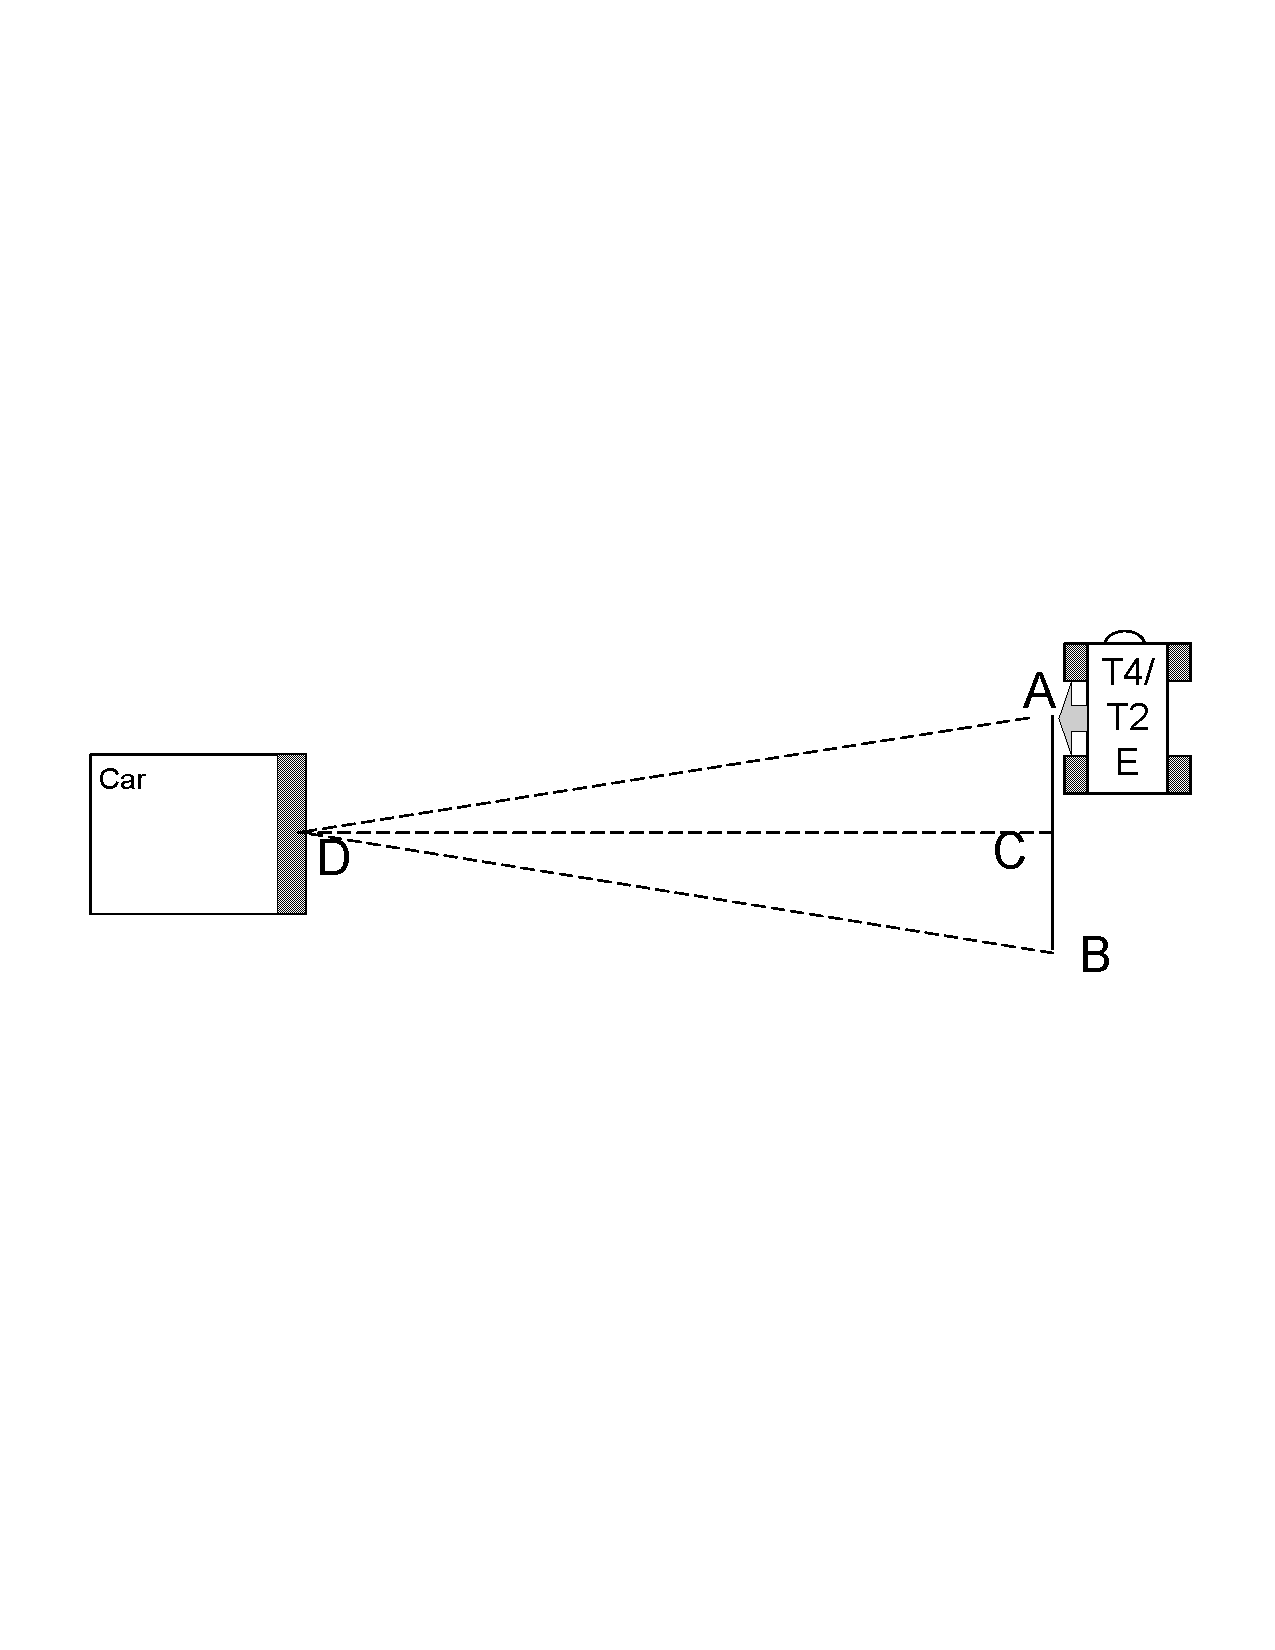
\includegraphics[width=0.5\textwidth]{LPRAng}\label{fig:LPRang}
\caption{Inspection distance and inspection angle of LPR system.}
\end{figure}

\begin{figure}[!htb]
%\begin{overpic}[scale=0.45,grid,tics=10]%
\begin{overpic}[scale=0.45]{DemoLPRAccuracy}
    \put(40,30){\huge\bf DEMO}
    \put(40,10){\huge\bf DEMO}
\end{overpic}
\caption{The accuracy rate of LPR system.}\label{fig:LPRacc}
\end{figure}


%\begin{figure}[!htb]
%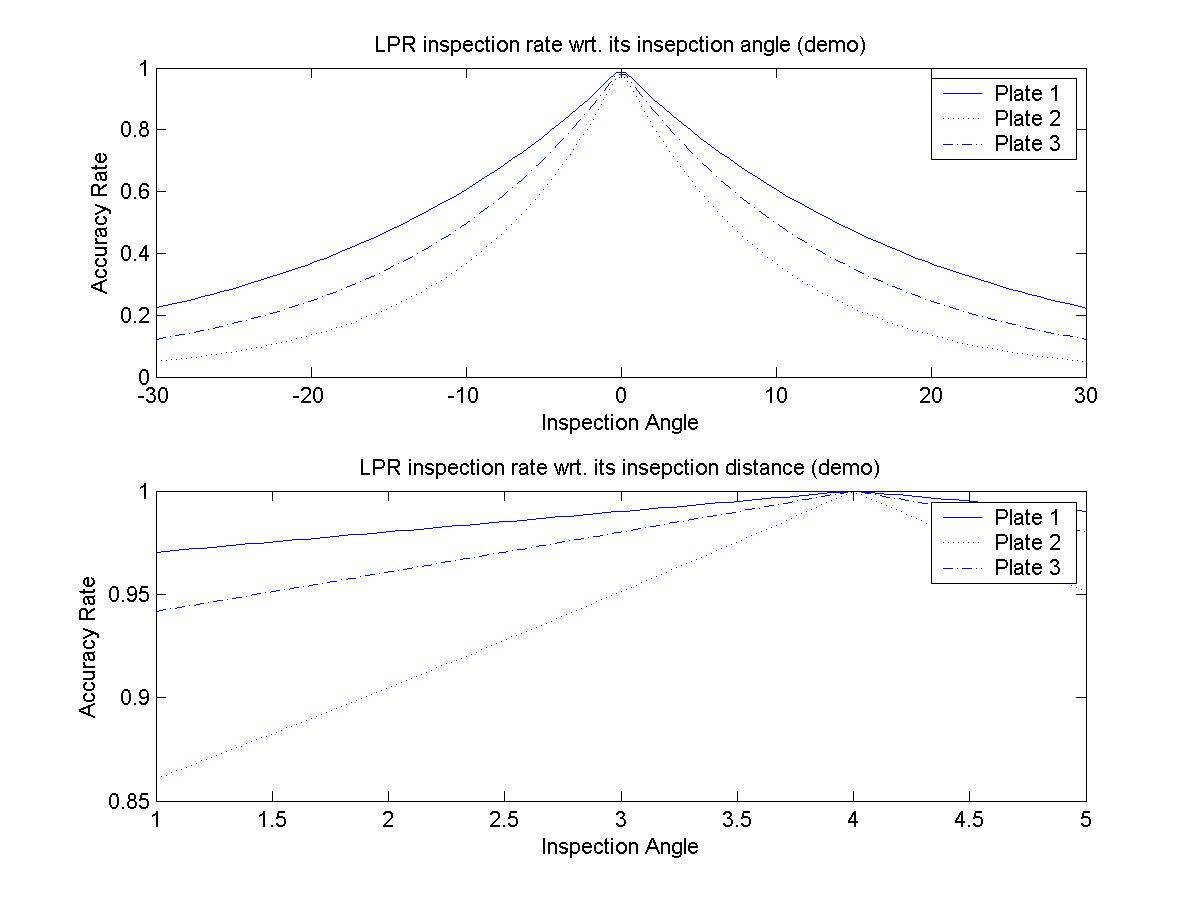
\includegraphics{DemoLPRAccuracy}
%\caption{The accuracy rate of LPR system.}\label{fig:LPRacc}
%\end{figure}

\begin{figure}
    \begin{minipage}{75mm}
    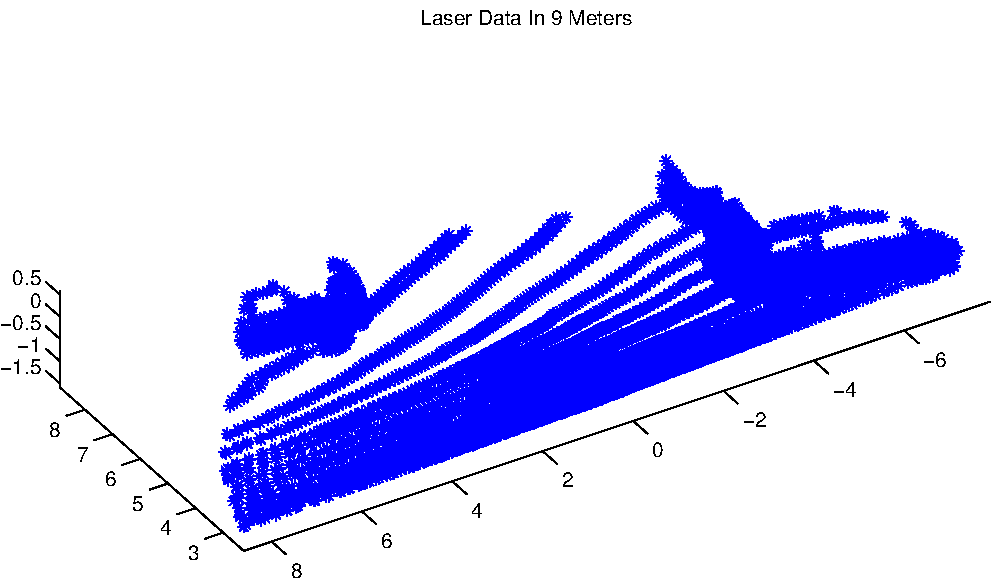
\includegraphics[width=\textwidth]{NearPts2}
    \caption{Collected laser data with tilt angle.}\label{fig:nearpts2}
    \end{minipage}
    \begin{minipage}{75mm}
    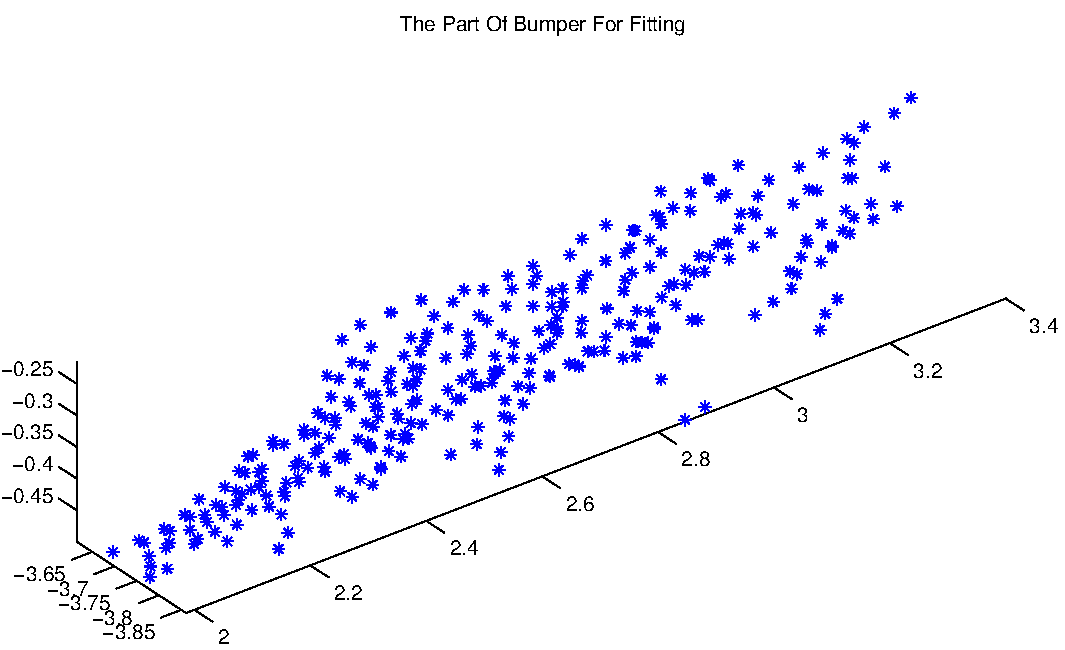
\includegraphics[width=\textwidth]{PartOfBumper}
    \caption{On Laser data set of a bumper.}\label{fig:bumper}
    \end{minipage}
\end{figure}~\com{later: fit bumper}


\subsection{Bumper Fitting Algorithms}
\com{Isotropic LMS vs. Hough}
    There are basically two fitting options: least mean square (LMS) type algorithms and Hough type transforms. In general, LMS is fast, but not as robust as Hough transform. If LMS was implemented on T4, a segmentation algorithm that can distinguish bumper and pedestrians, or ``in window objects'' is necessary for laser data pre-processing. To reduce the complexity, Hough type transforms was implemented on the real system. 

\com{Standard Hough}\com{Sparse Hough, and Log-Hough}\com{Efficiency analysis}
    Hough transform (HT) is a popular method for the extraction of geometric primitives \cite{HoughSurvey,Atherton99CHT}. Initially, it is only an approach for line detection. Later, many variants are developed to detect circle~\cite{Atherton99CHT}, ellipse~\cite{guil97lower}, or more complex binary patterns~\cite{guil96new}. A survey on Hough transform can be found in~\cite{HoughSurvey}. 

    Generally speaking, HT is robust to sensor noise at the expense of slow computation. The computational cost of the traditional HT is ${\cal O}(n^3)$ where $n$ is the number of data points. Though some efforts were made to speed up the HT algorithm~\cite{matas98progressive}, those fast strategies were developed generally for image data processing applications only. A SPHT algorithm was proposed in~\cite{Song02} for laser data fitting. In this paper, we will review it and compare the experiment results of SPHT and SHT.

%However, in our case, a 1D laser data set contains only {\em sparse}  binary information in the region of interest. Furthermore,  only a 1D array is required for laser data instead of a 2D  matrix for the image data. More importantly, the laser data set is  sequential or ordered. Taking these properties of laser data set into consideration, HT can be modified to reduce the computational time. 

\subsection{Sparse Hough Transform}

%In order to make the best use of the above mentioned features of laser scanner data set, here we propose a sparse Hough transform (SPHT) that fits better to the laser data processing problem. 
The Hough transform represents lines crossing a point by 
\begin{equation}
\rho = x \cos\theta + y \sin\theta,
\end{equation}
where $\rho$ and $\theta$ are the length of the normal and the angle of the normal with respect to the positive $x$-axis. $x$ and $y$ are the coordinates of a point of interest in the image.   $\rho$ and $\theta$ are quantified as an accumulator matrix. The value of each cell of the matrix represents how many times there is a line, denoted by $(\rho, \theta)$, passing a point in the image. The idea of SHT is to provide an equivalent but faster and less memory-demanding approach. %add new
The inputs and outputs of the SPHT algorithm are {\em exactly} the same as SHT, except that in sparse cases SPHT saves time and memory. Here sparse means both the number of data points and the number of the lines passing these points are small, which is true in our case. Basically, SPHT does not use a 2D array to record the votes. Instead, it uses a 1D  array for the  vote-counting. Since in sparse case, most lines passing one point are not the fitted line, we can compute only those lines that pass at least two points in the image. Transferring all the lines corresponding to one point in the image plane, as SHT does, will take extra computer memory and reduce the speed. 

    Based on the above considerations, we present an implementation of SPHT by the following pseudo-code list in Fig.~\ref{fig:spcode}.

 \begin{figure}[!htb]
\centering
    \begin{minipage}{130mm}
%\lstset{language={Matlab},breaklines=true,numbers=left,texcl=true,escapechar=@}
\lstset{language={Matlab},breaklines=true,labelstep=1,texcl=true,escapechar=@}
    \begin{lstlisting}{}
@(\texttt{Dat} is the input array; \texttt{Dat(n).x} is the $x$ value of the $n$-th point. @
@\texttt{Lines} is the output array that stores $(\rho,\theta)$ of the fitted lines.@
@\texttt{NumLen} is the number of the fitted lines.)@

@\texttt{NumLen=0}@
for i=1 to n-1
    for j=i+1 to n
        @$\alpha$ = atan($\frac{ Dat(i).y- Dat(j).y}{Dat(i).x - Dat(j).x} $)@
        @$\rho_0$ =Dat(i).x cos($\alpha$ -$\pi$/2) + Dat(j).y sin($\alpha-\pi/2$)@
        @$\theta$= $\alpha$-sign($\rho_0$) $\pi/2$@
        @$\rho=|\rho_0|$@
        @Cell$\theta$=floor($\theta$/$\Delta\theta$)$\times\Delta\theta$@
        @Cell$\rho$=floor($\rho/\Delta\rho$)$\times\Delta\rho$@
        @If the line $n$, where $n\in[1,\mbox{\tt NumLen}]$, is close enough to (Cell$\rho$,Cell$\theta$), increase the vote of Lines($n$) by one, otherwise {\tt NumLen=NumLen+1}, and add a line (Cell$\rho$, Cell$\theta$) to Lines with the vote equals to one.@
    end for
end for
    \end{lstlisting}
    \caption{Pseudo-code for sparse Hough transform}\label{fig:spcode}
    \end{minipage}
\end{figure}
    
%Figure~\ref{fig:spht} shows an example of the proposed SPHT. The SPHT transforms or fits  the raw data set to 2 lines. Actually,  the raw data could be interpreted as 2 lines,  or 2 lines plus a small transition arc, or even just one line. The exact segmentation depends on the resolution, or the threshold. For example, with a  precise laser sensor, we know  that the data in Fig.~\ref{fig:spht} cannot be a single line. However, with a low-precision sonar sensor, the target object might be just a single line. With a given sensor in real project, we should choose some reasonable thresholds by referring to the specifications of the sensors. Further discussions on the trade-off between sensor accuracy and the object fit accuracy can be found in~\cite{Goto98Efficient} and ~\cite{Goto00Design}.


\subsection{Analysis on Speed and Memory Size}
    In general, suppose that the angle resolution is denoted by $\Delta\theta$ and the normal resolution by  $\Delta\rho$. For SHT, $M\times N$ cells are required for the accumulator space, where $ M = \pi/\Delta\theta $ and  $N=\rho_{max}/\Delta\rho.$ In other words, the   memory size is $n\times M\times N$, where $n$ is the size of each cell. If there are $K$ valid points in the input data, the computation requirement is ${\cal O}(K\times M)$.

    For SPHT, if there are only $K$ valid points in the input, clearly, $K\ll M$ and $ K \ll N$. The maximum number of fitted lines will be $ K\times (K-1)/2$. The computation requirement is ${\cal O}(K\times (K-1)/2) $. The actual memory requirement depends on how many lines passing the data points in the input data. Normally, we expect that the number of lines, $L$, for our data is 2 to 4. It is easy to show that $L\leq K(K-1)/2$. 

    In~\cite{GieslerLogHough}, another scheme called Log-Hough transformation (LHT) was described. This algorithm is fast, with the complexity of ${\cal O}(n)$, and easy to implement. The authors introduced the concept of logarithmized cosine curve. For an arbitrary set of points, we can store the logarithmized cosine curve of a point of the set in a look-up table, then shift it by other parameters. The following is a comparison between the LHT and the SPHT:\\
\begin{itemize}
    \item Memory: The exact memory requirement of SPHT depends on the $L$, the line number. However, there is an upper bound of $K(K-1)/2$ units. For LHT, we need $k$ segments on the range of the accumulation space, where $ k=\lceil \log(\frac{r_1-r_0}{r_0})/\delta\rceil.$ The area of interest stretches from $r_0$ to $r_1$. $\delta$ is the angle resolution of the laser system.
    \item Resolution: The distance resolution of LHT is not uniform. The resolution of the near field is better than that of the far field. But the distance resolution of SPHT is uniform with respect to distance, with the resolution level the same as the range resolution of the laser scanner, e.g., the example in~\cite{GieslerLogHough} showed that if the range resolution of a laser scanner is 1cm, and the angle resolution is $0.5^\circ$, LHT will get a range resolution of 0.88cm for the objects at 50cm distance, and 16.6cm for the distance of 1000cm. For the same case, the distance resolution of SPHT will be always 1cm, no matter what the distance is.
    \item Complexity: The complexity of LHT is ${\cal O}(K)$ and that of SPHT is ${\cal O}(K(K-1)/2)$, where $K$ is the number of valid points. 
\end{itemize}    

    Figure~\ref{fig:SPHTLHT} shows the memory requirements, complexity and distance resolution of SPHT, LHT and SHT. Here we assume that the area of interest stretches from $r_0=50$cm to $r_1=1000$cm. The angular resolution $\delta$ is $0.5^\circ$. The distance resolution of the laser scanner is 1cm. Notice that the $x$ axis of the upper and middle subplots are scanning angles. In our application, instead of processing the data from $360^\circ$, we generally process only a narrow area, where SPHT has a good performance, as we can see from the figure. The upper figure shows that when the data set is very sparse, i.e., the angle of interest is narrow, SPHT demands the least memory. In the middle subplot of Fig.~\ref{fig:SPHTLHT}, we can estimate the rough speed of these algorithms based on their complexities.  SHT is very complex, while SPHT has less complexity, and LHT has the least complexity. Note: less complexity does not implies higher speed always. If an algorithm has less complexity than the other, it means the first one finally will be faster than the later one when the computation quantity increased. In the bottom subplot of Fig.~\ref{fig:SPHTLHT}, we can see that the range resolutions of SHT and SPHT are exactly the same. The memory and speed benefits from LHT is at the expense of a lower and distance-dependent resolution. 
    
    Because the basic feature of Hough type algorithms is ``voting'' on the accumulation space, they are progressive. To process each new income data point, the accumulation space must not be erased, and the fitting result will be improved if more data point comes. 

\begin{figure}[!htb]
    \centering
    \begin{minipage}{90mm}
    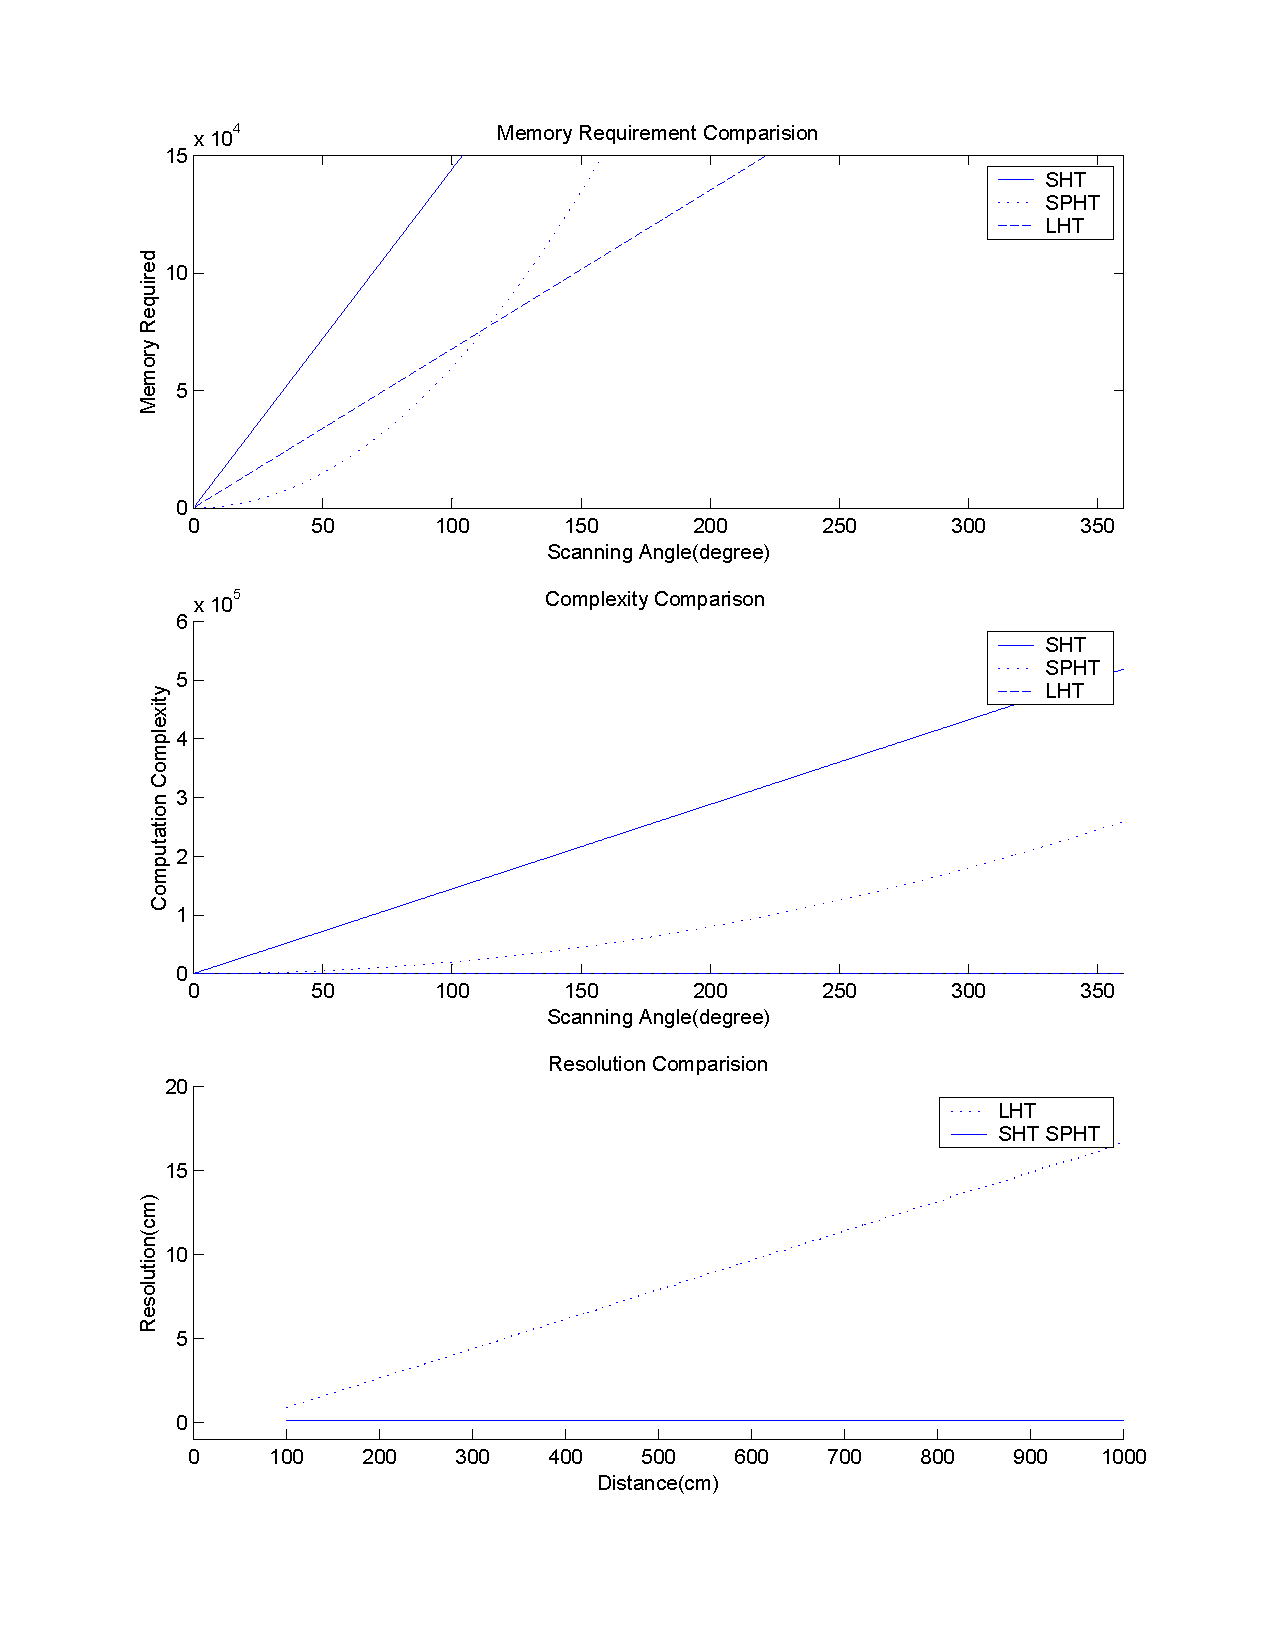
\includegraphics[width=\textwidth]{SPHTLHT}
    \caption{Comparison among SHT, SPHT and LHT.}\label{fig:SPHTLHT}
    \end{minipage}\hspace{3mm}
\end{figure}

%\begin{figure}[!htb]
%%    \begin{minipage}{0.45\textwidth}
%    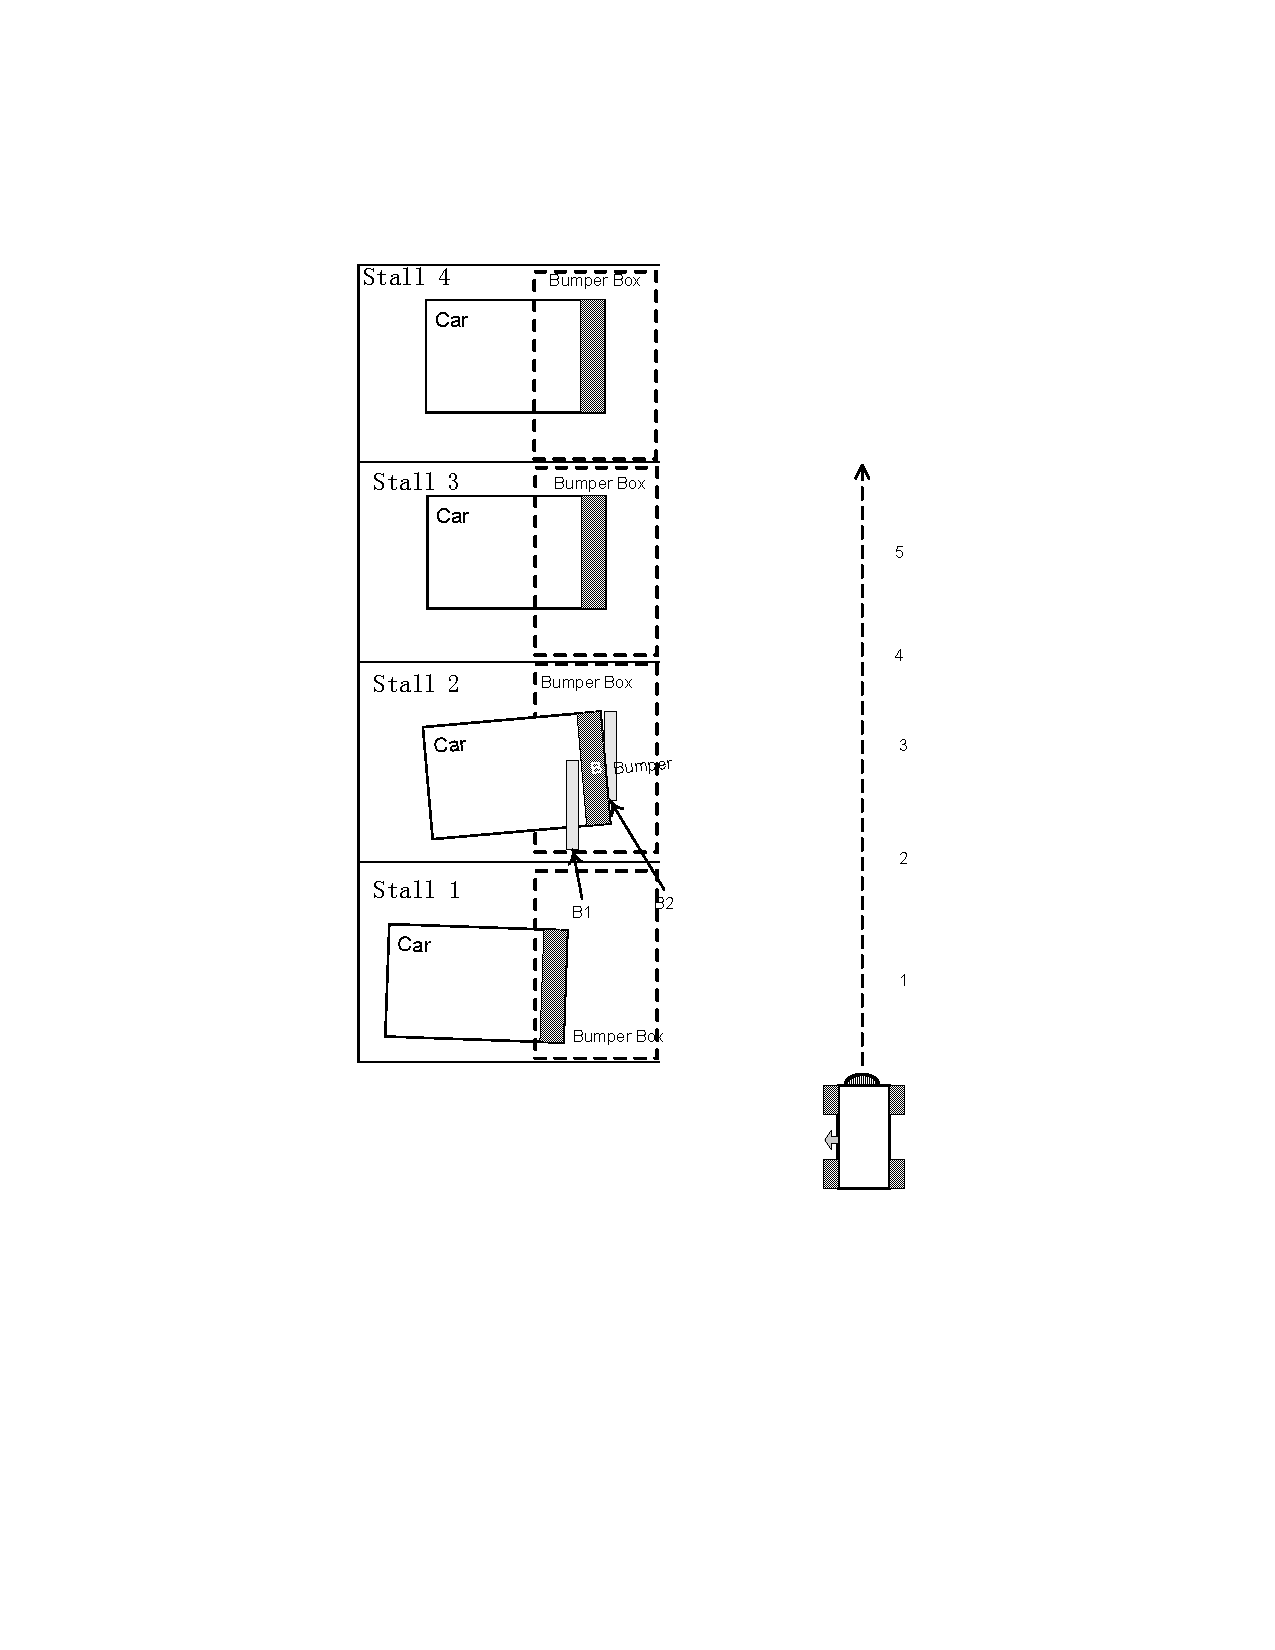
\includegraphics{Track}
%    \caption{License plate checking mission.}\label{fig:track}
%%    \end{minipage}
%\end{figure}
%
%\begin{figure}[!htb]
%%    \begin{minipage}{0.45\textwidth}
%    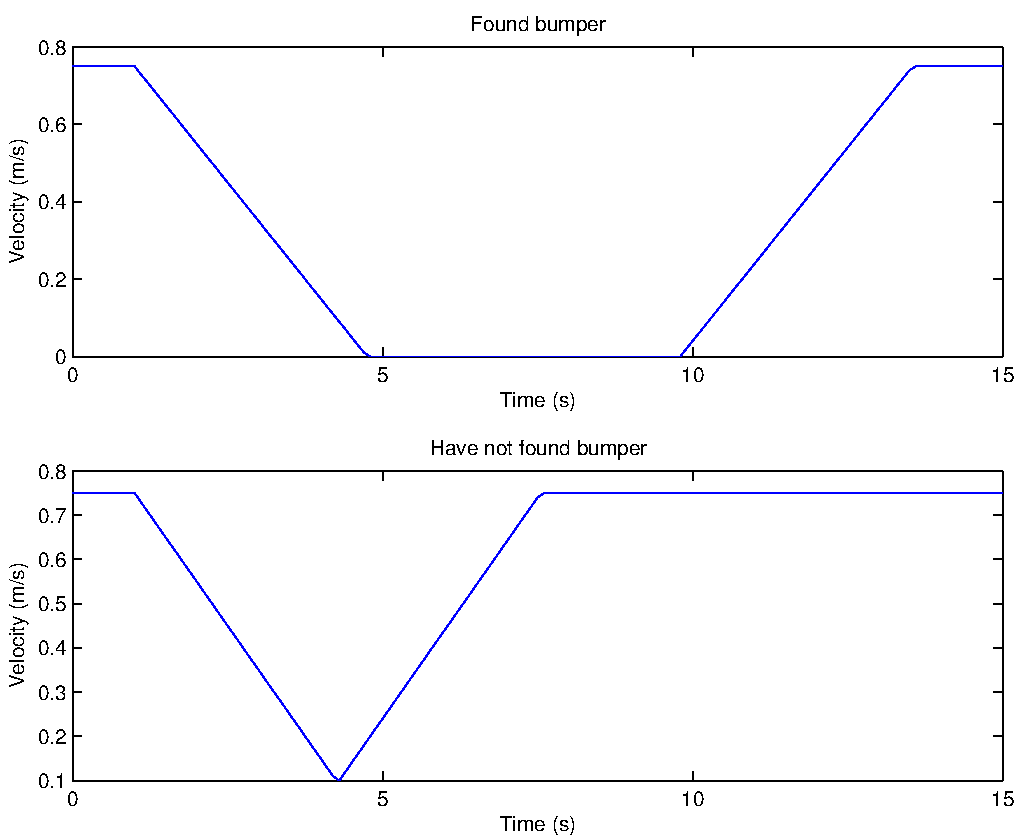
\includegraphics{FoundBumper}
%    \caption{The velocity behavior of bumper fitting.}\label{fig:foundb}
%%    \end{minipage}
%\end{figure}
\section{Experiment Results}\label{sec:exp}
\com{Positioning resolution}
%  C++ Speed  SPHT 0.1sec SHT 0.01+sec on 700mHz 256Mb desktop
%  Memory on Matlab SPHT 1*3  SHT 46*46 doubles 
%  res 9deg 6cm
    Figures~\ref{fig:OneSweepB} and \ref{fig:OneSweepL} are the example for SPHT bumper fitting. Figure~\ref{fig:OneSweepB} is one sweep of laser data on a vehicle bumper. After line fitting by SPHT, the result is plotted in Fig.~\ref{fig:OneSweepL}. The two circles represent the two laser data points that are believed as two ends of the bumper edge. When processing this example, the distance resolution was 6cm and angular resolution was 9$^\circ$. Except for the an array that stores the laser points, the SPHT just need 3 float variables, and SHT needs 46$\times$46 integer variables. When the C++ implemented of the two executing on a 700MHz, 256MB desktop, the SPHT took 0.1sec., and SHT took less than 0.02sec.. We did not implement LHT on T2E, because its variant resolution feature is complex for implementation, while its major advantage, fast speed, was not very urgent for our application. SPHT and SHT are fast enough. For the LHT approach, when robot was far from a specific bumper box, it needed less cells in accumulation space for bumper fitting. But while it was approaching the bumper box, more cells are requires. This takes time for implementation.

\com{Accuracy rate}
    Figure~\ref{fig:PklotMap} is a screen shot of part of the GUI on the workstation. The user had clicked \stall{6} to \stall{10} and sent T2E the LPR checking mission. This screen shot was taken when T2E almost finished the mission. The line in the middle of the figure is the track of T2E during the mission. The white edges in \stall{6}, \stall{7}, and \stall{10} are the fitted bumper lines. T2E had stopped before these stalls and triggered the \t4lpr application. 

    Figure~\ref{fig:T2EPlusGUI} overlapped a GUI screen shot (upper right) on a picture (background) in which T2E was moving in a parking lot. The returned license numbers were store in the hard disk of the workstation, in the mean time, they were displayed on a 3D perspective GUI. 

\begin{figure}
    \centering
    \begin{minipage}{70mm}
    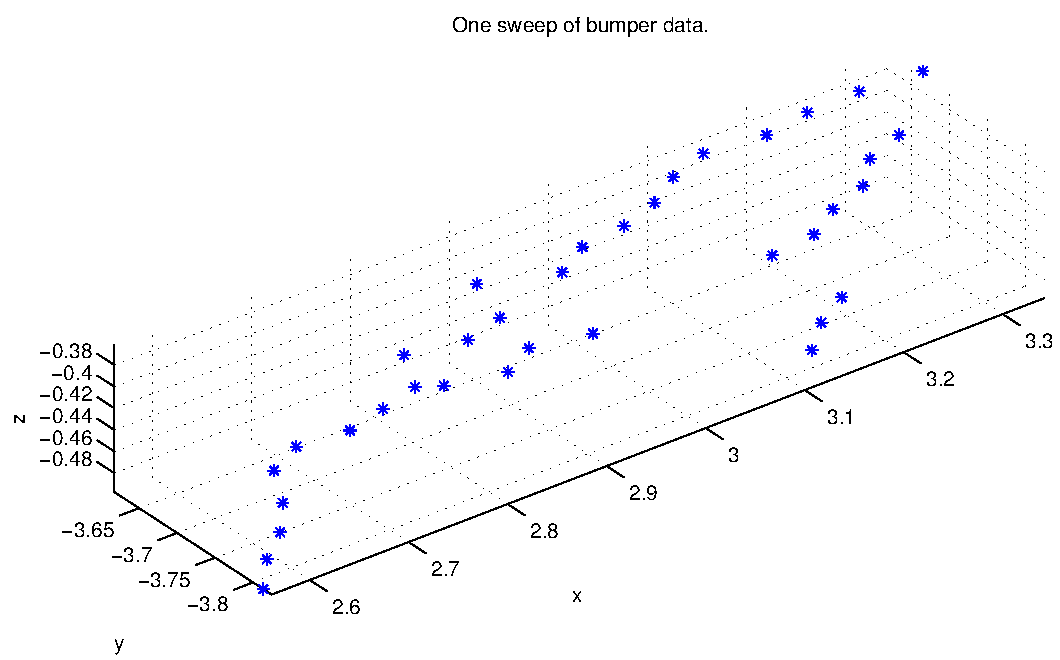
\includegraphics[width=\textwidth]{OneSweepBumper}
    \caption{One laser sweep on a bumper.}\label{fig:OneSweepB}
    
    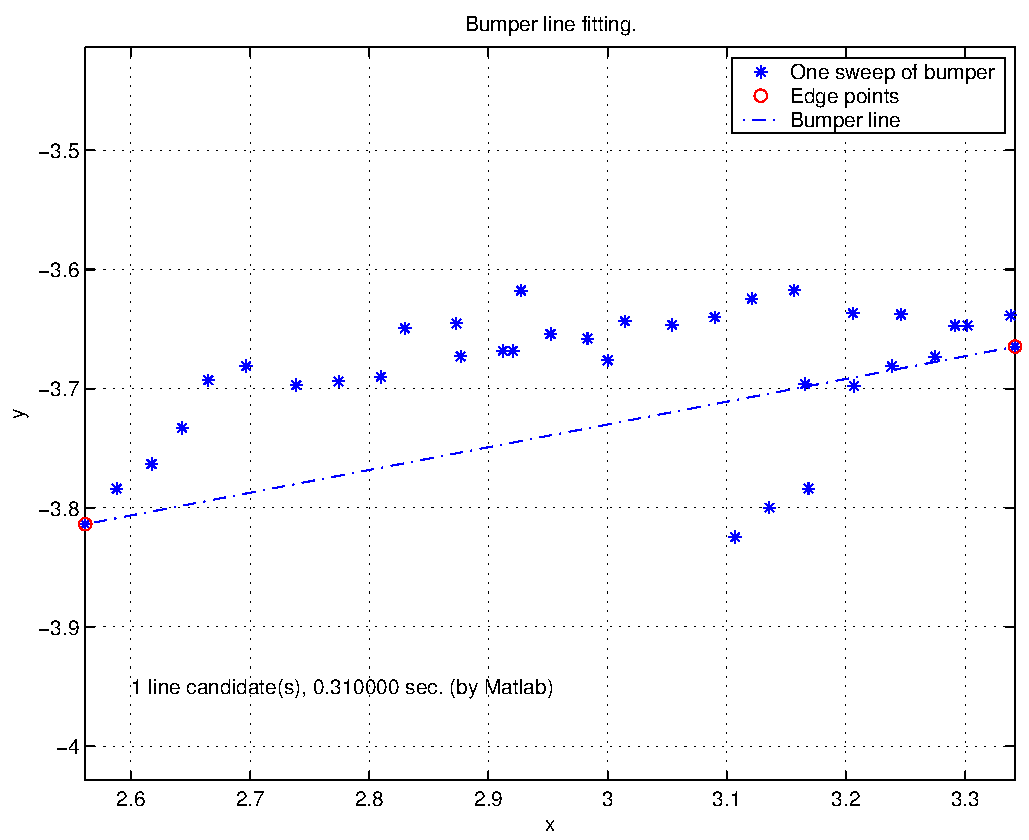
\includegraphics[width=\textwidth]{OneSweepBumperLine}
    \caption{One laser sweep on a bumper and its fitted bumper line.}\label{fig:OneSweepL}
    \end{minipage}
\end{figure}

\begin{figure}[!htb]
    \begin{minipage}{0.45\textwidth}
    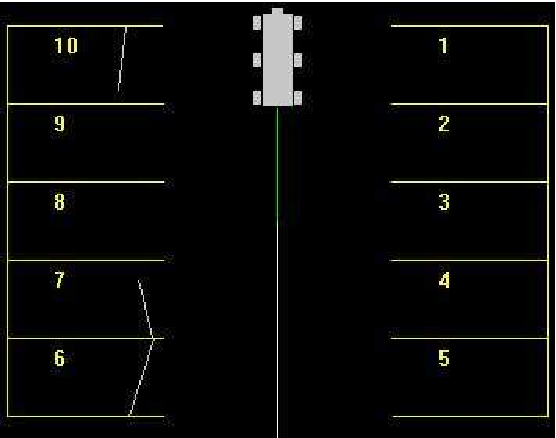
\includegraphics[width=\textwidth]{BumperLine}
    \caption{Bumper line on GUI.}\label{fig:PklotMap}
    \end{minipage}
    \begin{minipage}{0.45\textwidth}
    \includegraphics[width=\textwidth]{T2EPlusGUI}
    \caption{T2E executing bumper fit and check LPR mission.}\label{fig:T2EPlusGUI}
    \end{minipage}
\end{figure}



\section{Conclusion}\label{sec:con}
\subsection{Comments}
    In this paper presented a laser servoing system for precision motion control. Performed as the outer loop, this laser servoing system enhance the accuracy rate of an ODV robot LPR system by fitting bumpers. Since the platform T4 (T2E) robot is a complex autonomous system, there are many considerations for implementation details, such as the resources confliction, balance among different requirements, mission scheduling strategies. This paper carefully analyzed all requirements on the laser servoing system from those constrains, then proposed Hough transform based algorithms as the feedback processor. SHT and SPHT were implemented as the kernel algorithms for the bumper fitter. For this application, SHT is faster but takes more memory, and SPHT is vice versa: takes less memory but slower. Another bumper fitting algorithm, LHT, was discussed but not implemented. 

\subsection{Future Work}
    The concept of laser servoing might not be limited to LPR accuracy rate enhancement only. Instead, the similar algorithm might help robot to avoid danger, follow objects, or other autonomous missions. In future, the concept of laser servoing might be greatly expanded and extended. 
\bibliographystyle{spiebib}
\bibliography{SPIE03}%,\bibdir zhenPapers,\bibdir zhenBooks,\bibdir csois1,\bibdir csois2,\bibdir ZhenLocal}




\end{document} 